\pdfoutput=1
%
%
%
%
%
%
%
%
%
%
%
%
%
%
%
%
%
%
%
%
%
%
%
%
%
%
%
%
%
%
%
%
%
%
%
%
%
%
%
%
%
%
%
%
%
%
%
\documentclass[acmsmall,screen,nonacm]{acmart}
\settopmatter{printacmref=false}
%
%
\AtBeginDocument{%
  \providecommand\BibTeX{{%
    Bib\TeX}}}

%
%
%
%
%
\setcopyright{none}
%
\copyrightyear{2018}
\acmYear{2018}
\acmDOI{XXXXXXX.XXXXXXX}

%
\acmConference[Conference acronym 'XX]{Make sure to enter the correct
  conference title from your rights confirmation emai}{June 03--05,
  2018}{Woodstock, NY}
%
%
%
%
%
%
\acmPrice{15.00}
\acmISBN{978-1-4503-XXXX-X/18/06}


%
%
%
%
%
%

%
%
%
%
%
%
%
%
%
%
%
%

%
%
%
%
%
%
%
%
%
%
%
%
%
%
%


\usepackage{hyperref}
\usepackage{array}
\usepackage{todonotes}
\usepackage{proof}
\usepackage{stmaryrd}
\usepackage{xspace}
%
\usepackage{graphicx}

\usepackage{lipsum}
\usepackage[utf8]{inputenc}
%
\usepackage{blindtext}
\usepackage{listings}
\lstset{
  columns=fullflexible,
  numbers=left,
  basicstyle=\ttfamily,
  keywordstyle=\color{blue}\bfseries,
  morekeywords={mov,add,call},
  emph={rsp,rdx,rax,rbx,rbp,rsi,rdi,rcx,r8,r9,r10,r11,r12,r13,r14,r15},
  emphstyle=\color{green},
  emph={[2]cr3},
  emphstyle={[2]\color{violet}},
  morecomment=[l]{;;}
}
%
%
\newcommand{\setbackgroundcolour}{\pagecolor[rgb]{0.19,0.19,0.19}}  
\newcommand{\settextcolour}{\color[rgb]{0.77,0.77,0.77}}    
\newcommand{\invertbackgroundtext}{\setbackgroundcolour\settextcolour}
%
%
%
\usepackage{wrapfig}
\newtheorem*{remark}{Remark}

%
\usepackage{amsmath}

%
\usepackage{cleveref}
\crefformat{footnote}{#2\footnotemark[#1]#3}
\usepackage[T1]{fontenc}
\usepackage{fontawesome}
\usepackage[utf8]{inputenc}
\usepackage{iris}
\usepackage{mathpartir}
\renewcommand{\TirNameStyle}[1]{\hypertarget{#1}{\textsc{#1}}}
\newcommand{\RULE}[1]{\hyperlink{#1}{\textsc{#1}}\xspace}
\usepackage{xspace}
%
%
\newcommand{\sref}[1]{\S\ref{#1}}
\newcommand{\fref}[1]{Figure~\ref{#1}}
%
\def\etal.{\emph{et al.}}
\newcommand{\SL}{Separation Logic\xspace}
\newcommand{\spacelang}{SpaceLang\xspace}
\let\ar\rightarrow
\newcommand{\iProp}{\mathit{iProp}}
\newcommand{\lc}{$\lambda$-calculus\xspace}

%
%
\newcommand{\logical}{logical\xspace}
\newcommand{\logically}{logically\xspace}
\newcommand{\Logical}{Logical\xspace}
%
\newcommand{\tlfoff}[1]{\kw{pml4off}:#1}
\newcommand{\tltoff}[1]{\kw{pdpoff}:#1}
\newcommand{\tltwoff}[1]{\kw{pdoff}:#1}
\newcommand{\tlooff}[1]{\kw{ptoff}:#1}
\newcommand{\tpgoff}[1]{\kw{pageoff}:#1}
\newcommand{\lfoff}{\kw{pml4off}}
\newcommand{\ltoff}{\kw{pdpoff}}
\newcommand{\ltwoff}{\kw{pdoff}}
\newcommand{\looff}{\kw{ptoff}}
\newcommand{\pgoff}{\kw{pageoff}}
\newcommand{\crt}{\kw{cr3}}
\newcommand{\lt}{\kw{pdp}}
\newcommand{\ltw}{\kw{pd}}
\newcommand{\lo}{\kw{pt}}
\newcommand{\pg}{\kw{page}}
\newcommand{\tlf}[1]{\kw{cr3}:#1}
\newcommand{\tlt}[1]{\kw{pdp}:#1}
\newcommand{\tltw}[1]{\kw{pd}:#1}
\newcommand{\tlo}[1]{\kw{pt}:#1}
\newcommand{\tpg}[1]{\kw{page}:#1}
%
\newcommand{\modalPs}[1]{\vec#1}
\newcommand{\modalP}{P}
\newcommand{\modalQ}{Q}
\newcommand{\modaldefper}[2]{@[#1]\;\square\;#2}
\newcommand{\outsidemodaldefper}[2]{\square \; @[#1]\; #2}
\newcommand{\modaldef}[2]{@[#1]\; #2 }
\newcommand{\modaldefunfold}[2]{ #2 \; #1}
\newcommand{\modalstar}[2]{#1 \star #2}

%
\newcommand{\qfracone}{\kw{1}}
\newcommand{\qfracfot}{\kw{q}/512}
\newcommand{\qfracfots}{\kw{q}/512^{2}}
\newcommand{\qfracfotss}{\kw{q}/512^{4}}
\newcommand{\qfracfotsss}{\kw{q}/512^{8}}

\newcommand{\qfrac}{\kw{q}}
\newcommand{\qfractw}{\kw{q}/2}
\newcommand{\qfract}{\kw{q}/3}
\newcommand{\qfracf}{\kw{q}/4}
\newcommand{\naddr}{\kw{a}}
\newcommand{\vaddr}{\kw{va}}
\newcommand{\vpts}{\kw{v}}
\newcommand{\ppts}{\kw{p}}
\newcommand{\rpts}{\kw{r}}
\newcommand{\pfpointsto}[4]{#1\mapsto_{#4}\{#3\}\;#2}
\newcommand{\ppointsto}[3]{#1\mapsto_{#3}\;#2}
\newcommand{\npointsto}[4]{#1 / #2 \mapsto_{#4}\;#3}

\newcommand{\nfpointsto}[5]{#1\sim#2 \mapsto_{#5}\{#4\}\;#3}
\newcommand{\maskfour}{\textsf{l4M52}}
\newcommand{\maskfouroff}{\textsf{l4off}}
\newcommand{\maskthree}{\textsf{l3M52}}
\newcommand{\maskthreeoff}{\textsf{l3off}}
\newcommand{\masktwo}{\textsf{l2M52}}
\newcommand{\masktwooff}{\textsf{l2off}}
\newcommand{\maskone}{\textsf{l1M52}}
\newcommand{\maskoneoff}{\textsf{l1off}}
%
\newcommand{\mask}[3]{(#2\; #1 \; #3)}
\newcommand{\ft}{52}
\newcommand{\tw}{12}
\newcommand{\pointsto}{\mapsto}
\newcommand{\mystackrel}[2]{#2_{#1}}
\newcommand{\fpointsto}[1]{\mathrel{\mystackrel{#1}{\mapsto}}}
\newcommand{\pointedby}{\mapsfrom}
\newcommand{\vfpointedby}[1]{\mathrel{\mystackrel{#1}{\mapsfrom}}}
\newcommand{\vpointedby}{\mathrel{\mapsfrom}}
\newcommand{\mydagger}{\mathord{\dagger}}
\renewcommand{\ddag}{\mydagger\kern-0.8mm\mydagger}
\newcommand{\ddagsingleton}[1]{\ddag\{#1\}}
%
\newcommand{\ocloud}[3]{#3\;\text{\faCloud}^{#2}\,#1}
\newcommand{\cloud}[2]{\ocloud{#1}{#2}{#1}}
\newcommand{\pure}[1]{#1}
%
\newcommand{\rcpointedby}{\mathrel{\mapsfrom}}
\newcommand{\rcvpointedby}{\mathrel{\mapsfrom}}
\newcommand{\rcvfpointedby}[1]{\mathrel{\mapsfrom}_{#1}}
\newcommand{\nmaster}{m}
\newcommand{\nv}{n}
%
\newcommand{\centralinvariant}{I}
\newcommand{\generalentry}{\textsf{ent}}
\newcommand{\entryf}{\textsf{l4e}}
\newcommand{\entrytr}{\textsf{l3e}}
\newcommand{\entrytw}{\textsf{l2e}}
\newcommand{\entryo}{\textsf{l1e}}
\newcommand{\crthree}{\textsf{CR3}}
\newcommand{\paddr}{\textsf{pa}}
\newcommand{\vsome}{\_}
\newcommand{\vpage}{\textsf{v}}
%
\newcommand{\kw}[1]{\mathsf{#1}}

%

%
\newcommand{\pageptstosum}[2]{(#1+#2)}
\newcommand{\lvlsum}[2]{(#1+8*#2)}
\newcommand{\lvlbor}[1]{(#1 | \kw{w0}_{3})}
\newcommand{\Locsx}{\mathcal{W}_{16}}
\newcommand{\locsx}{\kw{w}_{16}}
\newcommand{\Locsz}{\mathcal{W0}_{16}}
\newcommand{\locsz}{\kw{w0}_{16}}

\newcommand{\Locn}{\mathcal{W}_{9}}
\newcommand{\locn}{\kw{w}_{9}}

\newcommand{\Loctw}{\mathcal{W}_{12}}
\newcommand{\loctw}{\kw{w}_{12}}
\newcommand{\Locsf}{\mathcal{W}_{64}}
\newcommand{\locsf}{\kw{w}_{64}}
\newcommand{\Locft}{\mathcal{W}_{52}}
\newcommand{\locft}{\kw{w}_{52}}

\newcommand{\rvsrc}{\kw{rv}_{\textsf{src}}}
\newcommand{\rgsrc}{\kw{r}_{\textsf{src}}}
\newcommand{\rv}{\kw{rv}}
\newcommand{\rg}{\kw{r}}
\newcommand{\rvdst}{\kw{rv}_{\textsf{dst}}}
\newcommand{\rgdst}{\kw{r}_{\textsf{dst}}}

\newcommand{\mvsrc}{\kw{rv}_{\textsf{src}}}
\newcommand{\mgsrc}{\kw{r}_{\textsf{src}}}
\newcommand{\mv}{\kw{rv}}
\newcommand{\mg}{\kw{r}}
\newcommand{\mvdst}{\kw{rv}_{\textsf{dst}}}
\newcommand{\mgdst}{\kw{r}_{\textsf{dst}}}

\newcommand{\Loc}{\mathcal{W}_n}
\newcommand{\loc}{\kw{w}_n}
\newcommand{\regset}{\kw{greg}}
\newcommand{\regvaltype}{\kw{regval}}
\newcommand{\reg}{\kw{r}}
\newcommand{\regval}{\kw{rv}}
%
\newcommand{\xs}{\mathit{xs}}
%
\newcommand{\pre}{\Phi}
\newcommand{\post}{\Psi}
\newcommand{\midpoint}{\chi}
%
\newcommand{\ql}{p}
\newcommand{\qv}{q}
\newcommand{\qw}{q'}
%
\newcommand{\lsv}{L}
\newcommand{\lsw}{L'}
%
\newcommand{\locs}{D}
\newcommand{\antecedents}{P}

%
%
\newcommand{\metaif}[3]{#1 \mathrel{?} #2 : #3}

%
\newcommand{\val}{v}
\newcommand{\vals}{\vec\val}
\newcommand{\wal}{v'}
\newcommand{\vunit}{()}
\newcommand{\vk}{k}
\newcommand{\vcode}[2]{\lambda#1.#2}
\newcommand{\vars}{\vec\var}

%
\newcommand{\lval}{\varrho}
\newcommand{\var}{x}
\newcommand{\sloc}{c}
\newcommand{\src}{r}
\newcommand{\dst}{s}
\newcommand{\dsts}{\vec\dst}
\newcommand{\lvals}{\vec\lval}

\newcommand{\ofs}{\mathit{o}}
\newcommand{\maddr}{\kw{maddr}}
\newcommand{\offs}{\kw{offset}}
%
\newcommand{\deref}{\mathord{*}}
\newcommand{\assign}{=}
\newcommand{\instr}{i}
\newcommand{\mvrr}{\kw{mvrr}}
\newcommand{\mvrmb}{\kw{mvrmb}}
\newcommand{\mvrmo}{\kw{mvrmo}}
\newcommand{\mvmrb}{\kw{mvmrb}}
\newcommand{\mvmro}{\kw{mvmro}}
\newcommand{\instrexpr}{\kw{ie}}
\newcommand{\instrs}{\ensuremath{\vec\instr}}
\newcommand{\iskip}{\ensuremath{\kw{skip}}}
\newcommand{\iseq}[2]{\ensuremath{#1; #2}}
\newcommand{\ising}[1]{\kw{sexec} (#1)}
\newcommand{\icall}[2]{\deref#1(#2)}
\newcommand{\ialloc}[2]{\deref#1 \assign \kw{alloc}\;#2}
\newcommand{\iload}[3]{\deref#1 \assign [\deref#2+#3]}
\newcommand{\istore}[3]{[\deref#1+#2] \assign \deref#3}
\newcommand{\iloceq}[3]{\deref#1 \assign (\deref#2 == \deref#3)}
\newcommand{\iconst}[2]{\deref#1 \assign #2}
\newcommand{\imove}[2]{\deref#1 \assign \deref#2}
\newcommand{\ialloca}[2]{\kw{alloca}\,#1\,\kw{in}\,#2}
\let\iallocaactive\ialloca
\newcommand{\ifork}[3]{\kw{fork}\,\deref#1\,\kw{as}\,#2\,\kw{in}\,#3}

%

\newcommand{\movctl}{\kw{movctl}}
\newcommand{\imreg}{\kw{imreg}}
\newcommand{\amode}{\kw{amode}}
\newcommand{\amodeb}[1]{\kw{amode}  #1}
\newcommand{\amodeo}[2]{\kw{amode} = #1 + #2}
\newcommand{\imov}[3]{#1 \; #2 \; #3}
%
\newcommand{\blk}{b}
\newcommand{\btuple}[1]{#1}
\newcommand{\bcell}[1]{\langle#1\rangle}
\newcommand{\bdeallocated}{\text{\normalfont\footnotesize\faBolt}}
\newcommand{\sz}[1]{\mathit{size}(#1)}
\newcommand{\replicate}[2]{#2^{#1}}
\newcommand{\pointers}[1]{\mathit{pointers}(#1)}

%
\newcommand{\storereg}{\sigma.\mathcal{R}}
\newcommand{\storemem}{\sigma.\mathcal{M}}
\newcommand{\storememstar}[1]{\sigma.\mathcal{M}^{*[#1]}}
\newcommand{\store}{\sigma}
\newcommand{\storeregprime}{\sigma'.\mathcal{R}}
\newcommand{\storememprime}{\sigma'.\mathcal{M}}
\newcommand{\storememprimestar}[1]{\sigma'.\mathcal{M}^{*[#1]}}

\newcommand{\storeprime}{\sigma'}

\newcommand{\logicalstore}{\theta}
\newcommand{\maxsize}{S}
%
\newcommand{\valid}[1]{\sz{#1}\leqmaxsize}
\newcommand{\available}[1]{\mathit{available}(#1)}
\newcommand{\closed}[1]{\text{$#1$ is closed}}
\newcommand{\related}[2]{#1\approx#2}

%
\newcommand{\predstore}{\pi}
\newcommand{\phinvariant}[2]{#1\bowtie#2}

%
\newcommand{\ectx}{K}
\newcommand{\hole}{[]}
\newcommand{\efill}[2]{#1[#2]}

%
\newcommand{\subst}[2]{[#2/#1]}
\newcommand{\readlval}[3]{#2(#1)=\bcell{#3}}
\newcommand{\writelvalsidecondition}[4]{
  #3(#1) = \bcell{\_}
}
\newcommand{\writelvalmaincondition}[4]{
  #4 = \mupd{#1}{\bcell{#2}}{#3}
}
%
%
%
%
\newcommand{\writelval}[4]{
  #4 = \langle #1 := #2 \rangle #3
}

\newcommand{\sexec}[4]{\kw{sexec}\(#1 #2 #3 #4\)}
\newcommand{\headstep}{\longrightarrow}
\newcommand{\cfg}[2]{#1\;/\;#2}
\newcommand{\hs}[4]{\cfg{#1}{#2}\headstep\cfg{#3}{#4}}
\newcommand{\hsfork}[5]{\cfg{#1}{#2}\headstep\cfg{#3}{#4}\mathrel{\textit{spawning}}#5}
\newcommand{\hsforknl}[5]{\begin{array}{@{}r@{}}\cfg{#1}{#2}\headstep\cfg{#3}{#4}\\\textit{spawning}\;#5\end{array}}
\newcommand{\hsnostore}[2]{\hs{#1}\store{#2}\store}
%
\newcommand{\gcSymbol}{\text{\normalfont\footnotesize\faTrashO}}
\newcommand{\gc}[2]{#1\mathrel{\gcSymbol}#2}
\newcommand{\headstepgc}{\mathrel{\;\gcSymbol\!\!\longrightarrow\,}}
\newcommand{\hsgc}[4]{\cfg{#1}{#2}\headstepgc\cfg{#3}{#4}}
\newcommand{\hsgcfork}[5]{\cfg{#1}{#2}\headstepgc\cfg{#3}{#4}\mathrel{\textit{spawning}}#5}

%
\newcommand{\alen}[1]{\mathord\mid#1\mathord\mid}

%
\newcommand{\varray}[1]{\begin{array}{@{}c@{}}#1\end{array}}
\newcommand{\starvarray}[1]{\bgroup\renewcommand{\star}{\\}\varray{#1}\egroup}
\newcommand{\BRACE}[1]{\left\{#1\right\}}
\newcommand{\BRACEvarray}[1]{\BRACE{\varray{#1}}}
\newcommand{\BRACEstarvarray}[1]{\BRACE{\starvarray{#1}}}
\newcommand{\triple}[3]{\{#1\}\;#2\;\{#3\}}
\newcommand{\atriple}[3]{\triple{#1}{&#2&}{#3}}
\newcommand{\vtriple}[3]{\varray{\{#1\}\\#2\\\{#3\}}}
\newcommand{\bigvtriple}[3]{\varray{\BRACEvarray{#1}\\#2\\\BRACEvarray{#3}}}
\newcommand{\bightriplehskip}{\;}
\newcommand{\bightriple}[3]{\BRACEstarvarray{#1}\bightriplehskip#2\bightriplehskip\BRACEstarvarray{#3}}
\newcommand{\bightriplex}[4]{\BRACEstarvarray{#1}\bightriplehskip#2\bightriplehskip\BRACE{\exists#3.\;\starvarray{#4}}}
\newcommand{\bigsupd}[2]{\BRACEstarvarray{#1}\supd\BRACEstarvarray{#2}}
%
\renewcommand{\wp}[2]{\mathit{wp}\;#1\;#2}

%
%
\let\ordinarystar\star
\DeclareMathOperator*{\Sep}{\scalerel*{\ast}{\sum}}
\newcommand{\bigast}[2]{\mathop{\textstyle\Sep}\limits_{#1}\,#2}
\let\ordinarybigast\bigast
\newcommand{\later}{\triangleright\;}

\newcommand{\logequiv}{\;\equiv\;}
\newcommand{\supd}{\Rrightarrow_\centralinvariant}
\newcommand{\fupd}{\Rrightarrow}
\let\ordinarysupd\supd
\newcommand{\iFalse}{\mathit{False}}
\newcommand{\iTrue}{\mathit{True}}

%
\newcommand{\singleton}[1]{\{#1\}}
\newcommand{\dom}[1]{\mathit{dom}(#1)}

%
\newcommand{\multiplicity}[2]{#1 \mathop{\text{\small\$}} #2}
\newcommand{\cardinal}[1]{|#1|}
%
\newcommand{\valoccs}[2]{#1 \mathop{\$} #2}

%
\newcommand{\singletonMap}[2]{[#1 := #2]}
\newcommand{\mupd}[2]{[#1 := #2]} %
\newcommand{\mext}[2]{[#1 \mathbin{+\!\!=} #2]} %

%
\newcommand{\JoinPointsto}{Join$\mapsto$}
\newcommand{\JoinPointedBy}{Join$\mapsfrom$}
\newcommand{\CovPointedBy}{Covariance$\mapsfrom$}
\newcommand{\ConfrontMapstoMapsfrom}{Confront$\mapsto\mapsfrom$}
\newcommand{\ConfrontDagMapsfrom}{Confront$\ddag\mathord{\mapsfrom}$}
\newcommand{\ZeroDiams}{Zero$\diamond$}
\newcommand{\JoinDiams}{Join$\diamond$}
\newcommand{\ZeroDag}{Zero$\ddag{}$}
\newcommand{\JoinDag}{Join$\ddag{}$}

\newcommand{\mathsmash}[1]{\ensuremath{\smash{#1}}}

%

%
\newcommand{\crval}{\kw{cr3val}}
\newcommand{\plusaddr}[2]{#1 + #2}
%

%

\newcommand{\listcopy}{\textit{copy}}
\newcommand{\self}{\textit{self}\,}
\newcommand{\destination}{\textit{dst}}
\newcommand{\source}{\textit{src}}
\newcommand{\etiquette}{\textit{tag}}
\newcommand{\head}{\textit{head}}
\newcommand{\tail}{\textit{tail}}
\newcommand{\res}{\destination'}
\newcommand{\callee}{\textit{f}\,}
%
\newcommand{\logval}{\mathit{v}}
\newcommand{\loglist}{\mathit{vs}}
%
\newcommand{\isListName}{\textit{isList}}
\newcommand{\isList}[2]{\isListName\;#1\;#2}
%
\newcommand{\lognil}{[]}
\newcommand{\logcons}[2]{#1 :: #2}
\newcommand{\loglistbrackets}[1]{[#1]}

%

%

\newcommand{\stackcreate}{\textit{create}}
\newcommand{\stackpush}{\textit{push}}
\newcommand{\stackpop}{\textit{pop}}
\newcommand{\isStack}[2]{\textit{isStack}\;#1\;#2}
\newcommand{\stack}{\textit{stack}}
\newcommand{\elem}{\textit{elem}}
\newcommand{\vns}{\mathit{vns}}
\newcommand{\nonreccallee}{\ensuremath{f}}

\newcommand{\coq}{\textsc{Coq}\xspace}
\newcommand{\HyLL}{\textsc{HyLL}\xspace}
\newcommand{\BI}{\textsc{BI}\xspace}
\newcommand{\BBI}{\textsc{BBI}\xspace}
\newcommand{\HyBBI}{\textsc{HyBBI}\xspace}
\newcommand{\iris}{\textsc{Iris}\xspace}
 \newcommand{\mytodo}[1]{%
  \todo[linecolor=white, bordercolor=white, textcolor=white]{#1}%
}


%
%
%
%
%
%

%
%
%
%
%
%
%
%
%
%
%
%

%
%
%
%
%
%
%
%
%
%
%



%
%
\begin{document}

%
%
%
\title{Modal Abstractions for Virtualizing Memory Addresses}
%
%
%
%
%
%
\author{Ismail Kuru}
\email{ik335@drexel.edu}
\author{Colin S. Gordon}
\email{csgordon@drexel.edu}
\affiliation{%
  \institution{Drexel University}
  \city{Philadelphia, PA}
  \country{USA}
}


%
%
%
%
%
%
\renewcommand{\shortauthors}{Kuru and Gordon}

%
%
%
\begin{abstract}
Operating system kernels employ virtual memory subsystems, which use a CPU's memory management units (MMUs) to virtualize the addresses of memory regions:
a logical (virtual) address is translated to a physical address in memory by the MMU based on
kernel-controlled page tables -- a hardware-defined sparse tree-map structure -- stored in memory, which itself is 
accessed by the kernel through virtual addresses.
Operating systems manipulate these virtualized memory mappings to isolate untrusted processes,
 restrict which memory is accessible to different processes, 
hide memory limits from user programs, 
ensure process isolation, implement demand-paging and copy-on-write behaviors for performance
and resource controls.
At the same time, misuse of MMU hardware can lead to kernel crashes.

Virtual memory management (VMM) code is a critical piece of general-purpose OS kernels, but verification of this functionality
is challenging due to the complexity of the hardware interface (the page tables are updated via writes to those
memory locations, using addresses which are themselves virtualized).
Prior work on verification of VMM code has either only handled a single address space, trusted significant
pieces of assembly code, or resorted to direct reasoning over machine semantics rather than
exposing a clean logical interface.

In this paper, we introduce a modal abstraction to describe
the truth of assertions relative to a specific virtual address space: [r]P indicating that P holds in the
virtual address space rooted at r. Such modal assertions 
allow different address spaces to refer to each other, enabling complete verification of instruction sequences
manipulating multiple address spaces. Using them effectively requires working with other assertions,
such as points-to assertions in our separation logic, as relative to a given address space.
We therefore define virtual points-to relations, which mimic hardware address translation,
relative to a page table root.
We demonstrate our approach with challenging fragments of VMM code showing that our approach
handles examples beyond what prior work can address, including reasoning about
a sequence of instructions as it changes address spaces.
All definitions and theorems mentioned in this paper including the operational model of a RISC-like fragment of x86-64, 
a simple language run on this operational model, and a logic as an instantiation of the Iris framework are mechanized 
inside Coq.
\end{abstract}

%
%
%
%
%
%
%
%
%
%
%
%
%
%
%
%
%
%
%
%
%
%
%
%
%
%
%
%

%
%
%
%

%
%
%
%

\maketitle

{
\theoremstyle{acmdefinition}
\newtheorem{assumption}[theorem]{Assumption}
}

%
\section{Introduction}
\label{sec:intro}
Virtual memory management lies at the core of modern OS kernel implementation. It is deeply intertwined with most other parts of a typical general-purpose OS kernel design, including scheduling, hardware drivers, and even the filesystem buffer cache. In writing the authoritative reference on the internals of the Solaris kernel, McDougall and Mauro went so far as to claim that ``\emph{the virtual memory sub-system can be considered the core of a Solaris instance, and the implementation of Solaris virtual memory affects just about every other subsystem in the operating system}''~\cite{mcdougall2006solaris}.
This makes rich support for verification the virtual memory management subsystem of an OS kernel critical to the correctness of every other piece of an OS or any software running atop it.

At its core, the virtual memory functionality of modern CPUs is about \emph{location virtualization}: the memory locations
(addresses) seen by most code are not, in fact, the exact location in physical memory where data reside. Instead these 
are \emph{virtual} addresses, which are mapped to actual physical resources by the cooperation of the hardware and OS. 
This is what enables separation of process memory resources:
the OS manipulates hardware functionality to ensure that any attempt by a process to access memory not explicitly granted 
to it by the kernel will fail. But this is complicated by the fact that 
%
%
control over these mappings of virtual to physical addresses is itself mediated by \emph{in-memory data structures}, 
which the kernel still accesses via virtual address, leading to indirect cycles.

Further complicating matters is that addresses themselves bear no information about which address space they originate 
from. For user processes this is of little concern, as these have access to only their own address space. But the kernel has
(or can grant itself) access to all address spaces. Mixing up addresses from different address spaces leads to severe bugs.
More concerning, keeping track of which \emph{assertions} hold in different address spaces during kernel verification is 
difficult: some assertions should hold across all address spaces, while others hold in only one, and others may hold in 
multiple but still not all.

This kind of context-dependent assertion, where a fact may be true in one address space but not others, has a modal flavor. 
We propose tackling the verification of virtual memory subsystems (and kernels more broadly) by adapting ideas from hybrid
modal logic, which can label assertions true under \emph{other, named} circumstances (i.e., in another address space) with a 
modality indexed by a name for that space (in our case, the root of the page tables for an address space). This offers a 
\textit{convenient} and \textit{powerful} way to \emph{modularly}
\begin{itemize}
\item isolate assertions specific to a particular address space,
\item explicitly state when an assertion is true across address spaces,
\item manipulate address spaces from within other address spaces, and
\item reason about change in address spaces.
\end{itemize}
These advantages make this approach to reasoning about virtual memory more flexible than prior program logic techniques~\cite{kolanski08vstte,kolanski09tphols}, 
which were only able to work with a single address space (the current address space on the CPU) because they were unable
to speak directly \emph{within the logic} about other address spaces.
%
%
%
%
%
%

\begin{itemize}
\item We develop these ideas in the form of a logic for working with virtual-address-space-relative assertions,
      implemented as an embedded separation logic within Iris~\cite{jung2018iris} separation logic.
\item We prove the soundness of our \textsf{vProp} logic with respect to a RISC-like fragment of \textsf{AMD64} instructions.
\item We verify simplified versions of several critical virtual-memory-related pieces of OS functionality, 
      including mapping  pages, and the assembly code for switching address spaces. 
      The latter in particular goes beyond the capabilities of prior work, and reveals unexpected
	subtleties.
\end{itemize}
 %
%
\section{Background}
\label{sec:background}
\subsection{Machine Model}
\label{sec:backgroundonmachinemodel}

In typical system configurations, all memory addresses seen by programs running on modern computers are \emph{virtualized}: the address observed by a running program generally will not correspond directly to the physical location in memory, and may not even correspond to a physical location that \emph{exists} in the machine. Instead, these \emph{virtual} addresses are translated to \emph{physical} addresses that correspond directly to locations in RAM. On most modern architectures, this translation is performed through cooperation of the hardware and OS kernel: while executing an instruction that dereferences a (virtual) address, the CPU's \emph{memory management unit} (\textsc{MMU}) implements an architecture-specific process of \emph{address translation}, resulting in a physical address used to access the cache\footnote{Technically, for performance reasons most caches are indexed with parts of the virtual address, but tagged with the physical data addresses, so cache lookups and address translations can proceed in parallel.} and/or memory-bus.

\begin{figure}
    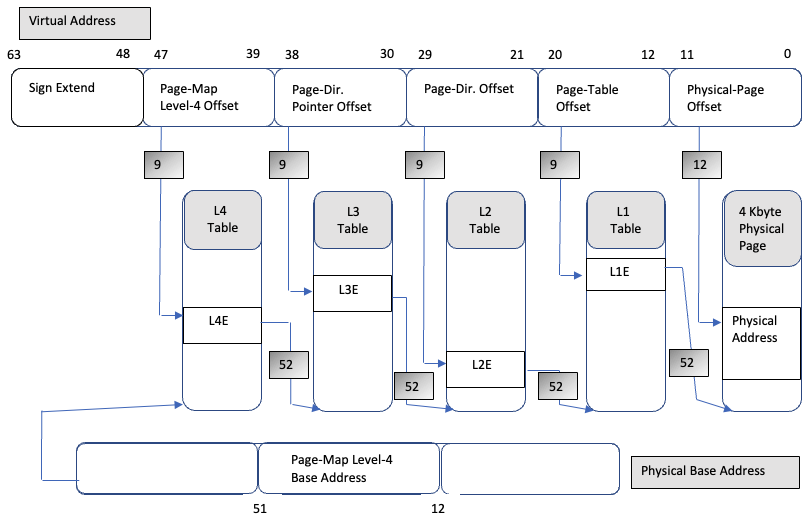
\includegraphics[width=\columnwidth]{pagetables.png}
    \caption{x86-64 page table lookups.}
    \label{fig:pagetables}
\end{figure}

On the x86-64 architecture, the input to the \textsc{MMU}'s address translation is a sparse hierarchical set of tables 
called \emph{page tables} (referring to pages of memory). As Figure \ref{fig:pagetables} (based on Figure 5-17 of the 
AMD64 architecture manual~\cite{amd64_manual_vol2}\footnote{While x86 up through its 32-bit incarnation were due to Intel,
the x86-64 architecture as a 64-bit extension to x86 was originally due to AMD. As a result, it is sometimes also referred to as the \texttt{amd64} architecture.}) shows, 
address translation proceeds by repeatedly taking designated slices of the virtual address and indexing into a table.
The final lookup in the page tables gives the base physical address of a page of physical memory, to which the low-order
bits of the accessed virtual address are added to determine the actual physical address retrieved. 
On x86-64, standard configurations use 4 levels of page tables, labelled levels 4 through 1, with lookups in the level 
1 page table resulting in the actual page of physical memory holding the requested data, and the low-order 12 bits 
being used to index into this page.\footnote{Technically levels 1--3 have designated names originating when there were 
fewer levels. We omit those names to avoid confusion for those not already steeped in the arcana of x86 history,
 and for greater consistency with the recent addition of a 5th level 
on the most recent processors, where levels 4 and 5 are simply known by their numbers. Our formalization
only deals with 4-level page tables, but is straightforwardly extensible to 5.}  
Because address translation 
traverses a series of tables, the translation process or algorithm is sometimes referred to as a \emph{page-table walk}. 
While Figure \ref{fig:pagetables} and most of our details are specific to the x86-64 architecture, ARMv8 (a.k.a.\ 
\texttt{aarch64}), RISC-V, and PowerPC use similar hierarchical page tables for address translation.

The entries of each table are 64 bits wide, but each points to a physical address aligned to 4KB (4096 byte) boundaries, which leaves 12 bits to spare to control a validity bit (called the \emph{present} bit), a read-write bit (which permits write access through the entry if and only if it is set), and a range of additional bits which can be used to control caching, write-through, and more. This paper will only consider the present bit (0), the read-write bit (1), and the accessed bit (5), which is set to 1 by the hardware every time an entry is used, allowing the OS to determine which pieces of memory are used or unused.

The page tables mapping virtual addresses to physical addresses are managed by the OS. Typically each process has its own 
virtual-to-physical mappings represented by its own page table, which the OS registers with the CPU by storing the (page-aligned)
physical address of the root of the page table tree (in our context, the start of the L4 table) in a 
specific register (\texttt{cr3}) as part of switching to a new process. 
Using different mappings, which map only disjoint portions of physical memory (with some exceptions in the next section) 
is how the OS ensures memory isolation between processes.

If an instruction is executed that accesses a virtual address that either has no mapping, or does not have a mapping permitting the kind of access that was performed (e.g., the instruction was a memory write, but the relevant address range was marked read-only in the relevant page table entry), the hardware triggers a \emph{page fault}, transferring control to a \emph{page fault handler} registered with the hardware by the OS, allowing it to take corrective action (described in the next section).

\subsection{Virtual Memory Managers}
\label{sec:backgroundonvmm}
Most OS kernels have a component called a \emph{Virtual Memory Manager} (VMM)\footnote{Not to be confused with Virtual 
Machine Monitor. In this paper we focus on non-hypervisor scenarios, but hardware virtualization extensions for both 
x86-64 and ARM make use of an additional set of page tables translating what a \emph{guest} considers to be its 
(virtualized) physical memory to actual physical memory. Our contributions should offer value in this scenario as well.}
which is responsible for setting up page table mappings and for taking action when a page fault occurs. Often, a page 
fault indicates a bug in a program --- for example, a null pointer dereference crashes a program not because the hardware
 designates it an error, but because most OSes refuse to map the first 4K worth of virtual addresses, so dereferencing 
\texttt{NULL} results in a page fault. In such cases, the OS will terminate the program.

In other cases the OS uses page faults to implement specialized functionality and optimizations. A key example of this is 
(confusingly) called \emph{paging}: saving room in physical RAM and avoiding unnecessary IO 
by waiting until memory addresses for code are accessed 
before copying them to RAM (in particular, saving process startup time); 
or copying memory that has not recently been accessed to disk 
(i.e., in a \emph{swap} file or partition) and marking those page table entries invalid so a future page fault will give 
the OS the chance to copy the relevant data back into memory when the program tries to access it again.

The key pieces of functionality a VMM must implement itself, or have available in another OS component (depending on 
design), are
adding a new page mapping (whether the mapped page contains zeros, file data, or swap data), and removing an existing 
page mapping.
While this initially sounds like relatively modest functionality whose implementation may be complicated by hardware 
subtleties, even these basic operations are actually quite intrictate.
Most notably, updates to the page tables are performed as writes to memory --- which are themselves subject to address translation.
In the case of changing the mappings for the currently-active set of page tables, the OS kernel is modifying the tables involved in its
own access of the tables.

%
%
%
%
%
%
%
%
%
%
%
%
%
%
%
%
%
%
%
%
%
%

%
%
%
%
%
%
%
%
%

Virtual memory concerns propagate to the OS scheduler, which is responsible for dealing with multiple 
address spaces, so must keep track of which virtual addresses are valid (and in what way) in which address spaces. 
Some virtual addresses are valid in only a single address space (e.g., a code address for a particular usermode 
process), while others are valid in all address spaces (e.g., kernel data structure pointers). 
The VMM must maintain some of these assumptions on behalf of the rest of the kernel, for example by guaranteeing that 
a certain range of virtual addresses (corresponding to the kernel's code and data) are valid in every address space.

\subsection{Modal Logic}
\label{sec:backgroundonmodallogic}
The problem of needing to keep track of things being true in some contexts and not in others is hardly unique to virtual 
memory management, and is the general insight behind most flavors of modal logic.

Most modal logics use unary operators on propositions to express that a logical claim $P$ is \emph{contingently} true 
in certain other circumstances, such as in other times~\cite{pnueli1977temporal} or places~\cite{gordon2019modal}. That is, for 
different modal operators $M$, $M(P)$ may mean that $P$ is true in another time or place (which may be a physical place 
like another network node~\cite{murphy2008type,gordon2019modal} or a conceptual place like a person's 
mind~\cite{hintikka1962knowledge}). A unifying concept across any modality is that they behave as applicative functors, 
typically satisfying (directly, or as a derived law, depending on the modality):
\[ (P\rightarrow Q) \rightarrow M(P) \rightarrow M(Q)\]
%
%
%
%
%
Many modalities, so-called \emph{normal} modalities also possess introduction rules of the form $P\rightarrow M(P)$, 
the classic example being that if $P$ is true, then $P$ is \emph{necessarily} true with the contingency picked up.%

Of particular interest for reasoning about virtual memory are modalities that permit \emph{naming} the alternate 
circumstances, prominently \emph{hybrid} modal logics~\cite{blackburn1995hybrid,areces2001hybrid}, which come equipped 
with assertions of the form $[\ell](P)$ indicating that $P$ is true in the specific alternate circumstance (Kripke world)
 named by the \emph{nominal} $\ell$. Note that a distinctive property of hybrid logics is that, rather than hiding
the points at which a modal assertion is evaluated inside the modality's definition, the choice of what world a modalized
assertion should be true in is chosen \emph{in the assertion itself}. This allows assertions to talk about not simply whether some other assertion
is true in some possible future or past world related in a fixed way to the current world, but to talk about \emph{arbitrary}
other worlds. This explicit naming of alternate worlds increases the power of modal logics~\cite{blackburn1995hybrid}, and is actually
necessary for completeness in classical separation logics~\cite{brotherston2014parametric}.

For our purposes, these are natural candidates to adapt for virtual memory management. We can reinterpret the notion of 
naming an alternate world slightly more loosely, and instead name \emph{address spaces} by the physical address of the 
page table root, since these structures are the physical representations of page tables. Thus in this paper we develop 
the notion that we can represent contingent truth of an assertion via $[r](P)$ indicating that $P$ holds in the address 
space rooted at physical address $r$.
The typical hybrid modality introduction rule, that $P$ and $\ell$ (indicating the current world is $\ell$) imply 
$[\ell](P)$, has a natural analogue: knowing $P$ and that the current address space is $r$ (i.e., that $r$ is the 
current \texttt{cr3} value) suggests a way to construct $[r](P)$. By the choice of \texttt{cr3} identifying the contingency, we can identify a fact
\begin{itemize}
  \item as a \textit{context} fact if its validity depends on \texttt{cr3} when it is outside the modality (i.e. modal context), and made \texttt{cr3} independent as a part of custom-tailored modal logic for virtual-memory: a truth representing a virtual-memory addressing depends \texttt{cr3} due to address-translation operation, is dependent on \texttt{cr3} in the ambient-logic (e.g. separation-logic), and is made \textit{independent} of the facts related to \texttt{cr3} by being introduced into the modal context under the assumption that it exhibits the knowledge on its validity with respect to \texttt{cr3} in the ambient logic.
  \item as a \textit{pure} fact as long as it does not \textit{necessarily} depend on any fact related to \texttt{cr3}: a truth representing a raw physical memory addressing, unlike virtual-address translation, does not need the \textit{knowledge} of \texttt{cr3}, therefore it can be introduce into the modal context as a pure fact
\end{itemize}

A relatively under-explored space of modal logics is the interaction of modal and substructural logics, 
in particular hybrid-style modalities in substructural logics, which has seen only minimal exploration~\cite{dovsen1992modal,restall1993modalities,d1997grafting,kamide2002kripke,licata2017fibrational} and no prior 
application. We develop our ideas in the Iris program logic~\cite{jung2018iris}, as a result exploring additional subtleties 
that arise where the modality itself may entail ownership of resources, as well as interactions between our hybrid-style 
modality and substructural rules.  For example, Iris contains a number of modalities that distribute over separating 
conjunction, or for which resources can freely move into the modality 
(e.g., $\blacktriangleright(P)\ast Q \wand \blacktriangleright(P\ast Q)$). In our setting some of these rules 
apply while others do not. For example, in our setting, an assertion that involves no modalities is interpreted as 
holding in the current (active-on-the-CPU) address space, so clearly cannot move into arbitrary other address spaces 
--- unless guarded by another address space modality.
%
%
%
%
%
%
%
%
%
%
%
 %
\definecolor{dkgreen}{rgb}{0,0.6,0}
\definecolor{ltblue}{rgb}{0,0.4,0.4}
\definecolor{dkviolet}{rgb}{0.3,0,0.5}

%
\lstdefinelanguage{Coq}{ 
    %
    mathescape=true,
    %
    texcl=false, 
    %
    morekeywords=[1]{Section, Module, End, Require, Import, Export,
        Variable, Variables, Parameter, Parameters, Axiom, Hypothesis,
        Hypotheses, Notation, Local, Tactic, Reserved, Scope, Open, Close,
        Bind, Delimit, Definition, Let, Ltac, Fixpoint, CoFixpoint, Add,
        Morphism, Relation, Implicit, Arguments, Unset, Contextual,
        Strict, Prenex, Implicits, Inductive, CoInductive, Record,
        Structure, Canonical, Coercion, Context, Class, Global, Instance,
        Program, Infix, Theorem, Lemma, Corollary, Proposition, Fact,
        Remark, Example, Proof, Goal, Save, Qed, Defined, Hint, Resolve,
        Rewrite, View, Search, Show, Print, Printing, All, Eval, Check,
        Projections, inside, outside, Def},
    %
    morekeywords=[2]{forall, exists, exists2, fun, fix, cofix, struct,
        match, with, end, as, in, return, let, if, is, then, else, for, of,
        nosimpl, when},
    %
    morekeywords=[3]{Type, Prop, Set, true, false, option},
    %
    morekeywords=[4]{pose, set, move, case, elim, apply, clear, hnf,
        intro, intros, generalize, rename, pattern, after, destruct,
        induction, using, refine, inversion, injection, rewrite, congr,
        unlock, compute, ring, field, fourier, replace, fold, unfold,
        change, cutrewrite, simpl, have, suff, wlog, suffices, without,
        loss, nat_norm, assert, cut, trivial, revert, bool_congr, nat_congr,
        symmetry, transitivity, auto, split, left, right, autorewrite},
    %
    morekeywords=[5]{by, done, exact, reflexivity, tauto, romega, omega,
        assumption, solve, contradiction, discriminate},
    %
    morekeywords=[6]{do, last, first, try, idtac, repeat},
    %
    morecomment=[s]{(*}{*)},
    %
    showstringspaces=false,
    %
    morestring=[b]",
    morestring=[d],
    %
    tabsize=3,
    %
    extendedchars=false,
    %
    sensitive=true,
    %
    breaklines=false,
    %
    basicstyle=\small,
    %
    captionpos=b,
    %
    columns=[l]flexible,
    %
    identifierstyle={\ttfamily\color{black}},
    %
    keywordstyle=[1]{\ttfamily\color{dkviolet}},
    %
    keywordstyle=[2]{\ttfamily\color{dkgreen}},
    %
    keywordstyle=[3]{\ttfamily\color{ltblue}},
    %
    keywordstyle=[4]{\ttfamily\color{dkblue}},
    %
    keywordstyle=[5]{\ttfamily\color{dkred}},
    %
    %
    %
    stringstyle=\ttfamily,
    %
    commentstyle={\ttfamily\color{dkgreen}},
    %
    literate=
    {\\forall}{{\color{dkgreen}{$\forall\;$}}}1
    {\\exists}{{$\exists\;$}}1
    {<-}{{$\leftarrow\;$}}1
    {=>}{{$\Rightarrow\;$}}1
    {==}{{\code{==}\;}}1
    {==>}{{\code{==>}\;}}1
    %
    {->}{{$\rightarrow\;$}}1
    {<->}{{$\leftrightarrow\;$}}1
    {<==}{{$\leq\;$}}1
    {\#}{{$^\star$}}1 
    {\\o}{{$\circ\;$}}1 
    {\@}{{$\cdot$}}1 
    {\/\\}{{$\wedge\;$}}1
    {\\\/}{{$\vee\;$}}1
    {++}{{\code{++}}}1
    {~}{{\ }}1
    {\@\@}{{$@$}}1
    {\\mapsto}{{$\mapsto\;$}}1
    {\\hline}{{\rule{\linewidth}{0.5pt}}}1
    %
}[keywords,comments,strings]

\section{Machine State \& Syntax}
\label{sec:syntax}
To develop our core logical ideas, we instantiate \textsf{Iris} with a simple language for streams of instructions, 
and a logical machine model corresponding to execution of x86-64 assembly instructions with virtual memory enabled on the 
CPU.

\subsection{Registers and Memory}
Programs we demonstrate in this paper requires accessing two types of computer resource: registers and memory.
A register identifier, $\reg$, is chosen from a fixed finite set of register identifiers, $\regset$. 
We use these identifiers $\reg$ for register names such as \texttt{rax}, \texttt{r8}, or \texttt{cr3}.
%
%
%
%
%
%
%
%
%
%
%
%
%
%
%
%
%
%
%
%
%
%
%
%
%
%
%
%
%
%
%
%
%
%
%
%
%
%
%
%
%
%
For clarity and ease of representation, we use machine words, $\loc \in \Loc$, with the subscripts showing the number of bits in a word,
for memory addresses, values, and offsets, rather than distinct location types that wrap machine words.
For example, $\kw{w}_{12}$ is a 12-bit word, which can be obtained for example truncating away 52 bits of a 64-bit word ($\kw{w}_{64}$).
\subsection{State}
\label{sec:state}
We represent the machine state mainly as a finite map of registers to register values and a map of word-aligned physical memory addresses 
to 64-bit physical memory values. 
Thus our states $\sigma$ include:
%
\begin{itemize}
%
\item A register map: $\sigma.\mathcal{R}: \kw{greg} \rightarrow_{\textrm{fin}} \kw{regval} $
\item A memory map: $\sigma.\mathcal{M}: \Locft \rightharpoonup_{\textrm{fin}} (\Loctw \rightharpoonup_{\textrm{fin}} \Locsf )$
\end{itemize}
Of particular note, \texttt{cr3}, the page table register, is included in the machine state.
%
\subsection{Instructions}
\label{sec:instructions}

\begin{figure}[t]
\begin{lstlisting}[language=Coq,mathescape]
 Definition translate (rtv: word 64) ($\sigma$: state) (w: word 64): word 64 + MemFail :=
      l4e $\leftarrow$ translate_top_level $\sigma.\mathcal{M}$ rtv w; 
      l3e $\leftarrow$ translate_from_l4e $\sigma.\mathcal{M}$ l4e w; 
      l2e $\leftarrow$ translate_from_l3e $\sigma.\mathcal{M}$ l3e w;
      l1e $\leftarrow$ translate_from_l2e $\sigma.\mathcal{M}$ l2e w;
      addr $\leftarrow$ translate_from_l1e $\sigma.\mathcal{M}$ l1e w;
      return concat (shift_dropn addr 3 three_lt64) low3.
\end{lstlisting}
\vspace{-1em}
\caption{\coq implementation of address translation (slightly simplified).}
\label{fig:coq_addr_translation}
\end{figure}

Programs in our logic are instruction sequences \instrs, which are formed by either a basic instruction \iskip, or prefixing an existing instruction
sequence with an additional instruction (\iseq\instr\instrs).
We model (and later, give program logic rules for) instructions for basic register moves, and reading and writing memory.
The latter require page table walks.
Figure \ref{fig:coq_addr_translation} gives a slightly simplified version of our address translation code in monadic style:
starting from the root page table address \textsf{rtv}, the virtual address \textsf{w} is either resolved to a physical address or an error is returned.
The full set of possible errors is not relevant to this paper; our logic is tailored for kernel code which should not fault,
so our proof rules guarantee no memory failures occur --- that the page table walk for any dereferenced address will succeed.

%
%
%
%
%

The main instructions we implement are variants of the x86-64 \lstinline|mov| instruction, which we format in Intel syntax (destination on the left, source on the right).
As expected \textsf{store} would be the update on the memory map entry
%
For memory operations, we treat
\[
\begin{array}{l}
  \hbox{(\TirNameStyle{WriteToMemFromReg})} \qquad
  \textsf{mov}~[r_m]~r_r \\
  \hbox{(\TirNameStyle{WriteToRegFromMem})} \qquad 
  \textsf{mov}~r_r~[r_m]
  \end{array}
  \]
which are realized by first translating the virtual-memory address of a memory location stored in $r_m$ to a physical memory location,
then updating those memory contents with the contents of register $r_r$ (\TirNameStyle{WriteToMemFromReg}) 
or loading the value at that physical memory location into the register $r_r$
(\TirNameStyle{WriteToRegFromMem}). 
%
Additional variants (such as instructions which access memory at a constant offset from the virtual address stored in a register) are also treated.

For register operations, we support moves back and forth between any pair of registers, though the \coq formalization splits these according to whether
the source or destination registers are standard data registers (e.g., \lstinline|rax|) or control registers (e.g., \lstinline|cr3|).
%
%
%
%
%
%
%
%
%
%
%
%
%
%
%
%
%
%
%
%
%
 %
\section{Program Logic for Location Virtualization}
\label{sec:logic}
%
\newcommand{\gammaPred}{\delta}
\newcommand{\gammaPreds}{\delta\textsf{s}}
\newcommand{\rtv}{\textsf{rtv}}
\newcommand{\qone}{\texttt{q1}}
\newcommand{\qtwo}{\texttt{q2}}
\newcommand{\qthree}{\texttt{q3}}
\newcommand{\qfour}{\texttt{q4}}

\newcommand{\sumwalkabs}[3]{
  \ownGhost\gammaPred{\authfrag{\singletonMap{#1}{(#2, #3)}}}
}

\newcommand{\sumapaces}[2]{
  \ownGhost\gammaPreds{\authfrag{\singletonMap{#1}{#2}}}
}
\newcommand{\ptableabswalk}[1]{\mathcal{A}\textsf{bsPTableWalk}(#1)}
\newcommand{\ptablestore}{\theta}

We derive a program logic (a separation logic) supporting the following stances and constraints:
\begin{enumerate}
\item \textit{address-spaces as modal contexts}: Assertions in our logic are context-dependent,
  in the sense that their truth depends on which address space they are used in, due to the need to support virtual points-to assertions.
\item \textit{sharing}: The physical location backing a virtual address's storage is located (during a page table walk) through a 
      set of physical page-table (L4-L1 page-tables) acceses that are shared amongst different virtual addresses (specifically,
      those on the same page of memory\footnote{of in the case of L2 or higher levels of tables, within a given broader region.}).
      This sharing imposes constraints on definiting points-to assertions
      in terms of physical (L4-L1) page-table memory accesses
\item \textit{context-agnostic-resources}: each virtual address is valid under a certain address-space, 
      but it does not represent this \textit{knowledge} of its address-space. 
      That is, assertions are not explicitly tagged with their address space validity
\item \textit{updating address-space mappings}: We present logical abstractions to enable 
      updating not only pages of typical data in memory, but also page tables themselves.\footnote{Prior work relied on unfolding operational semantics
      to verify page table updates.}
\item \textit{explicitly-modal assertions}: Our logic includes a means to talk about facts being true
      in another address space
\item \textit{address-space switch as changing the "World" of truth}: Switching from one address-space to another logically
      becomes a simultaneous introduction-and-elimination of a pair of modal assertions (for different address spaces)
\end{enumerate}

The first viewpoint, that the truth of an assertion is relative to an address space, has far-reaching consequences.
Therefore, as a first step, we work entirely in a pointwise lifting of Iris's base BI logic,
essentially working with separation logic assertions indexed by a page table root as a $\mathcal{W}_{64}$
(Figure \ref{fig:vprop}), which we call $\textsf{vProp }\Sigma$; this is the (\textsc{Coq}) type of assertions in our logic.
Most constructs in Iris's base logic are defined with respect to any BI-algebra (of \textsc{Coq} type \lstinline|bi|), so automatically
carry over to our derived logic.
However, be must still build up from existing Iris primitives to provide new primitives that depend on the address space --- primarily the notion
of virtual points-to.

\begin{figure}[t]
\begin{lstlisting}[language=Coq]
  Definition vProp  $\Sigma$ : bi := word 64 -b> iPropI  $\Sigma$.
  \end{lstlisting}
\caption{$\textsf{vProp }\Sigma$: Root-Address Indexed Address-Space Proposition}
  \label{fig:vprop}
\end{figure}

\subsection{Base Points-To Assertions}
\label{sec:pointsto}
We build up our context-dependent assertions from two basic types of assertions that do not care about address spaces.

\paragraph{Register points-to} 
The assertion $\textsf{r}\;\mapsto_{\textsf{r}}\{q\}\;\textsf{rv}$ ensures the ownership of the register $\rg$ naming the register value $\rv$. 
The fraction $\qfrac$ with value 1 asserts the unique ownership of the register mapping, and grants update permission on it, 
otherwise, any value $0 < \qfrac <1$ represents partial ownership granting readonly permission on the mapping.

\paragraph{Physical memory  points-to} The soundness proofs for our logic's rules largely center around page-table-walk accesses as in Figure \ref{fig:coq_addr_translation},
 where (inside the helper functions) we need to split a 64-bit word representing entries in these tables into 52-bit segments
which specify the physical page number of another page in the walk, and 12-bit segments containing various control bits.
For this reason we have two notions of physical points-to facts. The primitive notion closest to our machine model is:
\[ \textsf{w1} \ \sim \ \textsf{w2} \mapsto_{\textsf{a}} \; \{\textsf{q}\} \; \textsf{v} \]
In this form, we see that \textsf{w1} (a $\mathcal{W}_{52}$) essentially selects a 4KB page of physical memory,
and \textsf{w2} (a $\mathcal{W}_{12}$) is an offset within that page.
%
%
%
From this we can derive a more concise physical points-to when the split is unimportant:
%
\[\textsf{w} \mapsto_{\textsf{p}} \{q\} \textsf{ v} \stackrel{\triangle}{=} (\textsf{drop 12}~w) \ \sim \ (\textsf{bottom 12}~w)\mapsto_{\textsf{a}} \textsf{ v} \]

\begin{figure*}
  \begin{lstlisting}[language=Coq]
 Definition $\vaddr\mapsto_{\textsf{t}}\{\textsf{q}\}\; \vpage$ : vProp $\Sigma$ := 
  $\exists_{\textsf{l4e l3e l2e l1e}} \ldotp$  $\ulcorner$ aligned $\vaddr \urcorner \ast$ L4_L1_PointsTo($\vaddr$ l4e l3e l2e l1e paddr) $\ast$ paddr $\mapsto_{p}\{\mathsf{q}\} \vpage$.
 Definition L4_L1_PointsTo (maddr l4e l3e l2e l1e paddr :word 64) : vProp $\Sigma$ :=
 $\lambda$ cr3val.
  $\ulcorner$ entry_present l4e $\land$ entry_present l3e $\land$ entry_present l2e $\land$ entry_present l1e$\urcorner$ $\ast$
  (l4M52 maddr cr3val) $\sim$ (l4off maddr cr3val) $\mapsto_{a}$ {q1}  l4e  $\ast$
  (l3M52 maddr l4e) $\sim$ (l3off maddr l4e)  $\mapsto_{a}$ {q2}  l3e $\ast$ 
  (l2M52 maddr l3e) $\sim$ (l2off maddr l3e) $\mapsto_{a}$ {q3}  l2e $\ast$
  (l1M52 maddr l2e) $\sim$ (l1off maddr l2e) $\mapsto_{a}$ {q4}  l1e.
\end{lstlisting}
\vspace{-1em}
\caption{A Strong Virtual Points-to Relation}
  \label{fig:strongvirtualpointsto}
\end{figure*}



\subsection{An Overly-Restrictive Definition for Virtual Memory Addressing}
\label{sec:overly-restrictive}
A natural definition for a virtual points-to that depends on the current address space is to
require that in order for a virtual address \textsf{va} to point to a value \textsf{v}, the assertion contains
partial ownership of the physical memory involved in the page table walk that would translate \textsf{va} to
its backing physical location --- with locations existentially quantified since a virtual points-to should not assert
\emph{which} locations are accessed in a page table walk.
Figure \ref{figure:strongvirtualpointsto} gives such a definition.
It asserts the existence of for page table entries, one at each translation level, and via \lstinline|L4_L1_PointsTo|
asserts from the current \lstinline|cr3| value, taking the offsets from \textsf{va} (as in Figure \ref{fig:pagetables})
to index each level, finding the existentially quantified entries in each level, 
ending with the L1 entry, whose physical page base is added to the page offset of \textsf{va} to obtain the physical address
 --- and there (\lstinline|addr_L1(va,l1e)|) in physical memory, is the value.
Most of the definition lives directly in \textsf{vProp}, using the separation logic structure lifted from Iris's \textsf{iProp}.

\lstinline|L4_L1_PointsTo| works by
chaining together the entries for each level, using the sequence of table offsets from the address being translated to index
each table level, and using the physical page address embedded in each entry.
For example, 
  the first level address translation to get the L4 entry (\lstinline|l4e|) 
  uses the masks \textsf{l4M52} with the current \lstinline|cr3| to get the 
  physical address of the start of the L4 table,
  and \textsf{l4off} with the virtual address being translated to compute the correct offset within that table.
  Then at that physical location is the appropriate entry in the L4 table \textsf{l4e}.
  Subsequent levels of the page table walk work similarly.
The statement of these assertions is simplified by the use of our split physical points-to assertions, since
each level of tables is page-sized.\footnote{We do not address superpages and hugepages in this paper.}
This helper definition is also a more explicit \textsf{vProp}, explicitly binding a value for \lstinline|cr3| and using it
to start the translation process.


%
%
%
%
%
%
%
%
%
%
%
%
%
%
%
%
%
%
%
%
%
%
%
%

This solution is in fact very close to that of \citet{kolanski08vstte}, who define a separation logic from scratch in \textsc{Isabelle/HOL},
where the semantics of all assertions are functions from pairs of heaps and page table root values to booleans.\footnote{
  This was a typical explicit construction at the time; their work significantly predates Iris.
}
Our solution removes some restrictions in this definition by further abstracting the handling of address translation.

\subsection{Aliasing/Sharing Physical Pages}
  \label{sec:sharingpages}  
  One might have already observed that the virtual points-to definition shown in Figure \ref{fig:strongvirtualpointsto} 
  is too strong to specify some operations a virtual memory manager may need to do, such as
  move one level of the page table to a different physical location while preserving all virtual-to-physical mappings.\footnote{
    x86-64 hardware, like other architectures, includes a feature (which we do not formalize assertions for) to
    replace an L1 page table address in an L2 entry with a pointer to a \emph{larger} 2MB page (called super-pages), 
    or replace an L2 page table address in an L3 entry with a pointer to a 1GB page (called huge-pages).
  }
   To speak more concretely, the fractional permissions on the page-table-walk assertion ($\textsf{L}_{4}\_\textsf{L}_{1}\_\textsf{PointsTo}$ in Figure \ref{fig:strongvirtualpointsto}) 
  ensure fractional ownership of the four physical page table entries accessed by the hardware during address translation,
  as well as the physical memory holding the data of the virtual points-to.
  However, this formulation stores knowledge of the page table walk's details with ownership of the backing physical
  memory.
  Updating any of these mappings (e.g., moving the page tables in physical memory, as in coallescing for
  superpages or hugepages)
  would require explicitly collecting all virtual points-to facts that traverse affected entries.
  It is preferable to permit the page tables themselves to be updated independently of the virtual points-to assertions,
  so long as those updates preserve the same virtual-to-physical translations.
\newcommand{\vale}{\textsf{val}}
\begin{figure*}
\[
\begin{array}{l}
    \vaddr\mapsto_{\textsf{v}}\{\textsf{q}\}\;\vale : \mathsf{vProp}~\Sigma \stackrel{\triangle}{=} \\
    \quad
    \exists \paddr\ldotp
    \exists \delta\ldotp
    \underbrace{\lambda\mathit{cr3val}\ldotp\sumapaces{\mathit{cr3val}}\delta}_\text{\begin{tabular}{c}Find ghost map for this\\address space\end{tabular}} \ast 
  \underbrace{\sumwalkabs\vaddr\qfrac\paddr }_\text{\begin{tabular}{c}Fractional ownership of \\virt-to-phys translation\end{tabular}}\ast 
  \underbrace{\paddr \mapsto_{\mathsf{p}} \vale}_\text{\begin{tabular}{c}Value at\\physical location\end{tabular}}
\end{array}
\]
\caption{Virtual-Pointsto for Sharing Pages}
  \label{fig:virtualpointstosharing}
\end{figure*}  

  Intuitively, the definition in Figure \ref{fig:strongvirtualpointsto} is too strong because the virtual points-to
  assertion there tracks too much information: when writing programs that access memory via virtual addresses,
  most code does not care \emph{which physical memory locations are involved in address translation}: it only cares
  that virtual address translation would succeed. The necessary information about the physical page table walk
  must still be tracked, but can be tracked separately from the virtual points-to assertion itself.

  We take the approach of separating the physical page-table-walk pointsto ($\textsf{L}_{4}\_\textsf{L}_{1}\_\textsf{PointsTo}$ in Figure \ref{fig:strongvirtualpointsto}) 
  from the virtual pointsto relation. 
  To do so, we take advantage of an Iris construction which permits tracking a map in ghost state that maps
  virtual addresses to the physical addresses they translate to, and has for each key in the map (i.e.,
  each virtual address) a token. Updating the virtual-to-physical (ghost) mapping for a virtual address $va$
  requires full ownership of the token. In addition, we keep an invariant that for each $va\mapsto pa$ mapping
  in this map, there are \emph{physical} resources sufficient to ensure that address translation for $va$
  will resolve in the hardware to $pa$. But these physical resources, which specify \emph{which} physical locations
  are involved in the page table walk, are now separated from but consistent with
  the knowledge that such resources exist (which is embodied by the token for $va$, which tracks that $va$ maps to $pa$
  in the ghost map). Thus we can store the token which summarizes the translation and ensures it exists in the virtual
  points-to, and keep the ghost map and the invariant that every mapping in the ghost map has corresponding physical resources
  for translation in a separate global invariant.

  %
  %
  In Iris this is realized by using an authoritative resource algebra: there is a single \emph{authoritative} global copy of the (ghost)
  map caching virtual-to-physical address translations, and for each entry a read only \emph{partial} ownership of that key-value pair.
  The resource algebra itself is instantiated as:
  \[\mathcal{A}\textsf{bsPTableWalk} \stackrel{\triangle}{=} \textsc{Auth} (\; \mathcal{W}_{64} \;\rightarrow_{\textrm{fin}} \;  ( (\textsc{Frac }, \mathord{+}) \times (\textsc{Agree } \Loc,\mathord{=}) ))\]
We replace the physical
 $\textsf{L}_{4}\_\textsf{L}_{1}\_\textsf{PointsTo}$
with
fragmental ownership of the ghost-map ($ \sumwalkabs\vaddr\qfrac\paddr$),
 whose ownership just ensures that the virtual address ($\vaddr$) is mapped to a page (referenced by $\paddr$)


We place the authorative ownership $\mathcal{A}\textsf{PTableWalk}$ of the ghost-map in a per-address-space invariant
($\mathcal{I}$\textsf{ASpace} in Figure \ref{fig:peraspaceinvariant}) whose ownership, when combined with the
fraction stored in the virtual points-to, permits changes in the virtual-to-physical translations.
By itself, it allows changes to the page tables as long as they do not change the overall mappings from virtual
to physical addresses.



  \begin{figure*}
\[
\begin{array}{l}
  \mathcal{I}\textsf{ASpace}(\ptablestore,m)\stackrel{\triangle}{=} \textsf{ASpace\_Lookup}(\ptablestore,m) \ast \\
 \qquad\qquad\qquad \bigast{(\vaddr, \textsf{paddr})\in \ptablestore}{\exists\;(\textsf{l4e l3e l2e, l1e, paddr})\ldotp \textsf{L}_{4}\_\textsf{L}_{1}\_\textsf{PointsTo}(\vaddr\textsf{, l4e, l3e, l2e, l1e, paddr})} \\
  \textsf{ where } \\
   \textsf{ASpace\_Lookup} (\ptablestore,m) \stackrel{\triangle}{=} \lambda\textsf{ cr3val} \ldotp \; \exists \gammaPred \; \ldotp \ulcorner m \; !!\; \textsf{cr3val} = \textsf{Some } \gammaPred \urcorner \ast
    \ownGhost\gammaPred{\authfull{\ptableabswalk\ptablestore}}
  
\end{array}
\]
\caption{Global Address-Space Invariant with a fixed global map of address-space names $m$}
  \label{fig:peraspaceinvariant}
  \end{figure*}

Another major change is that, because our logic is the first to explicitly address the existence of multiple address spaces,
the ghost map of virtual-to-physical translations (identified by the ghost name $\delta$ in Figure \ref{fig:virtualpointstosharing}
 \emph{for each address space}. This means we also require a way to locate the map for the current address space
from the current root page table pointer stored in \lstinline|cr3|.

Figure \ref{fig:peraspaceinvariant} describes the resources for each address space, which are collected
for the full address space, but separated from virtual points-to assertions.
$\Theta$ is the logical map from virtual addresses to the physical addresses they should translate to, 
for the \emph{current} address space, corresponding to the currently installed page tables (the ones
indicated by \lstinline|cr3|). In Figure \ref{fig:virtualpointstosharing}, the existentially-quantified $\delta$
is the ghost name for the authoritative copy of this map (again, for the current address space).
$m$ is the (full) logical map from the various page table bases to ghost names for the 
per-address-space mappings like $\Theta$.
It is the full version of the map named by the ghost name $\delta{}s$ in
Figure \ref{fig:virtualpointstosharing}; there is only one such map in the system.
This is why Figure \ref{fig:virtualpointstosharing} asserts there is some ghost name in that (global) map
for the current address space.
The global map itself is tracked by a resource algebra 
\[\mathcal{A}\textsf{spaces} \stackrel{\triangle}{=} \textsc{Auth} (\; \mathcal{W}_{64} \;\rightarrow_{\textrm{fin}} \;  ( (\textsc{Frac }, \mathord{+}) \times (\textsc{Agree } \textsc{GhostName},\mathord{=}) )) \]


$\mathcal{I}\textsf{ASpace}(\Theta,m)$ is then the resources for the current address space:
It ensures that the current address space is valid (it has an entry in $m$, whose corresponding
authoritative map matches $\Theta$), and asserts ownership of the appropriate fractional ownership
of the physical page table walk for each virtual-to-physical translation in $\Theta$ (for the current address space).



  
Figure \ref{fig:logicaladdrspace} depicts the relationships between these pieces, for a single
address space.
The invariant for the currently active address space (solid round square labelled as 
$\mathcal{I}$\textsf{ASpace} in Figure \ref{fig:logicaladdrspace}) asserts authorative ownership (i.e. 
update capability), $\ownGhost\gammaPred{\authfull{\ptableabswalk\ptablestore}}$, of the ghost map $\Theta$
describing virtual-to-physical address translations
-- shown as a solid-round-head arrow to $\mathcal{A}\textsf{PTableWalk}$.
Each virtual points-to assertion (dashed round square labelled as \textsf{Virtual PointsTo}
 in Figure \ref{fig:peraspaceinvariant})
asserts fragmental ownership of the ghost map $\Theta$, $\sumwalkabs\vaddr\qfrac\paddr$,
shown via the dashed-diamond-head arrow to $\mathcal{A}\textsf{PTableWalk}$. Specifically, it asserts that
the virtual address the virtual points-to assertion concerns corresponds to some physical address.
There exists only one persistent authorative ownership 
($\ownGhost\gammaPred{\authfull{\ptableabswalk\ptablestore}}$) which collects the fragmental 
ghost page-table-walk mapping ($\sumwalkabs\vaddr\qfrac\paddr$),
 shown as double-ended solid arrow 1 to N imposing the update protocol.

\begin{figure}
   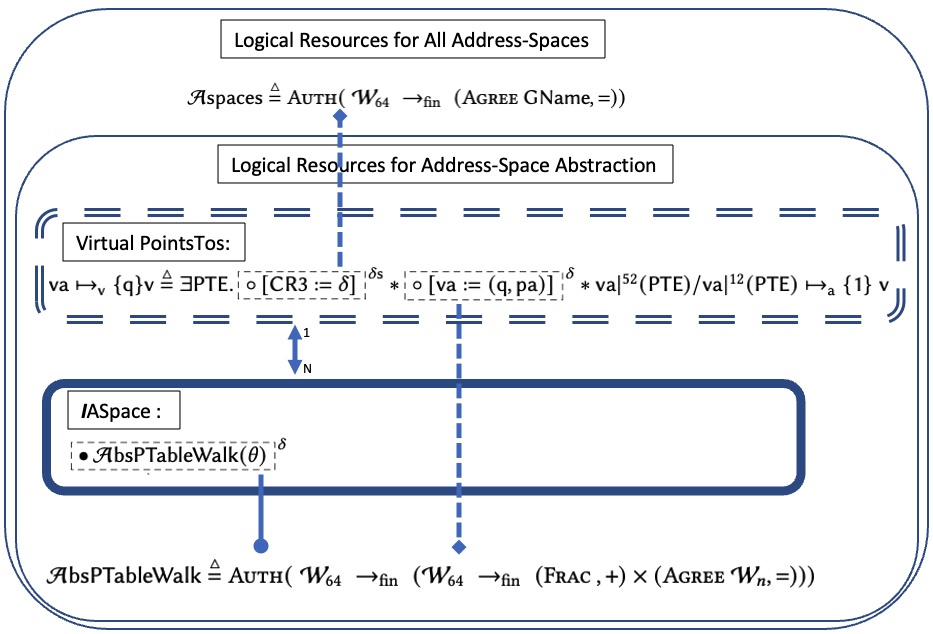
\includegraphics[width=0.75\columnwidth]{logical_addr_space.png}
  \caption{Logical Resources of Address-Space Abstraction (1 Address Space)}
  \label{fig:logicaladdrspace}
  \end{figure}

\paragraph{From A Single Address Space to Many}
In principle the resources from each individual address space should be collected into a single
shared invariant, and for each memory access,
a fragment of this corresponding to $\mathcal{I}\textsf{ASpace}(\Theta,m)$
for the current address space should be extracted from this global resource, used to prove correctness of the
memory access, and put back.
In this paper we focus on the middle section, explicity identifying resources for each
address space. The reason for this is that in practice, this global resource is also
the place where kernel-specific assumptions, such as guaranteeing that certain virtual address range
was mapped in all address spaces, would be enforced. This paper focuses on the
reasoning principles behind the virtual memory access, and we leave the use of this within a larger
kernel to future work.

\subsection{Address-Space Management}
\label{sec:aspacemanagement}
So far, we have introduced logical abstractions for a single address space. However, virtual memory management
implementations typically handle more than one address-space,
and doing this requires assertions which talk about other address spaces, and means to switch address spaces.
%

%

%
%
%

%
\begin{figure}
\[
  \begin{array}{r@{\qquad}l}
    \hbox{(\TirNameStyle{ModalAddressSpace})} &
         [r](\mathsf{P}) \;: \mathsf{vProp} \; \Sigma \; \stackrel{\triangle}{=} \; \lambda \_,\; \mathsf{P}~\mathsf{r}.\\
    \hbox{(\TirNameStyle{ModalAddressSpaceMono})} & (\textsf{P} \vdash \textsf{Q}) \vdash  ([r](\textsf{P}) \vdash  [r](\textsf{Q}))\\
    \hbox{(\TirNameStyle{ModalAddressSpaceSep})} & [r](\textsf{P} \ast \textsf{Q}) \dashv\vdash ([r](\textsf{P}) \ast [r](\textsf{Q})\\
    \hbox{(\TirNameStyle{ModalAddressSpaceAnd})} &   [r](\textsf{P}\land \textsf{Q}) \dashv\vdash [r](\textsf{P})\land [r](\textsf{Q})\\    
    \hbox{(\TirNameStyle{ModalAddressSpaceOr})} &    [r](\textsf{P}\lor \textsf{Q}) \dashv\vdash [r](\textsf{P})\lor [r](\textsf{Q})\\   
    %
    \hbox{(\TirNameStyle{ModalAddressSpaceFact})} &  \textsf{Fact P} \stackrel{\triangle}{=} \;\forall \; ,r \; r' \ldotp  \textsf{P r} \dashv\vdash \textsf{P r'}\\
    %
    %
    \hbox{(\TirNameStyle{ModalAddressSpaceFactIntroElim})} 
    &\textsf{Fact P} \vdash  ([r](\textsf{P}) \dashv\vdash (\textsf{P}) %
  \end{array}
  \]
  \caption{Other-space Modality and Its Laws}
  \label{fig:modaldef}
  \end{figure}
Figure \ref{fig:modaldef} gives the definition of our modal operator for asserting truth of a modal
(address-space-contingent) assertion \emph{in another address space}, which we call
the \emph{other-space} modality. The definition itself is not
particularly surprising --- as our modal assertions are semantically predicates on a page table root (physical)
address, the assertion $[r](P)$ is a modal assertion which ignores the (implicit) current page table root,
and evaluates the truth of $P$ as if $r$ were the page table root. This simple definition is 
what we need in order for assertions in one address space to talk about assertions in another.

The inspiration for this assertion comes from hybrid logic~\cite{blackburn1995hybrid,areces2001hybrid,goranko1996hierarchies,gargov1993modal},
which as mentioned earlier uses as modalities the names of worlds in a Kripke model to state
that an assertion is true in that specific world.
Conceptually the address space rooted at some physical address (intended as the start of an L4 table)
is a distinct world, and it makes sense to name it by referring to the root of the
supporting page table structure. However, rather than explicitly building a Kripke model for our
assertions, we inherit them by lifting the model of our ambient logic, Iris.

This assertion is also useful in proofs: we can prove that this modality follows certain useful laws, and that it interacts with
a class of assertions which are true regardless of which address space they are evaluated in.
The other-space modality distributes over the various separation logic connectives, and follows the rule of
consequence.
We also define a class of \textsf{vProp}s we call \textsf{Fact}s, which are those assertions
which ignore their address space entirely.
Physical points-tos and register value assertions, when treated as \textsf{vProp}s, are \textsf{Fact}s.
\textsf{Fact}s can move in and out of other-space modalities freely.



  
%
%
%
%
%

%
%
%
%
%

%
%
%

%

%

%
%
%
%
%
%

\subsection{The Impact of Changing Address Spaces on Modal Assertions}
%
%
\label{sec:issues}
An important subtlety arises with supporting \lstinline|mov|s into \lstinline|cr3|. Consider the hypothetical rule
\begin{mathpar}
\inferrule[Broken]{ }{
  \{P \ast \textsf{cr3}\mapsto_{r} \;r_1 \ast r \mapsto_{r} \;r_2 \ast [r_2](Q)\}
  \texttt{mov}~\texttt{\%cr3},~r%
  \{[r_1](P) \ast \textsf{cr3} \mapsto_{r} r_2 \ast r \mapsto_{r} r_2 \ast Q\}
}
\end{mathpar}
which is slightly simplified (by dropping per-address-space resources) for clarity in making the following point.
This rule captures the intuitive change of address space in a Hoare triple.
The problem with this is that it interacts quite poorly with the traditional frame
rule and the modal flavor of virtual points-to assertions.
If we abbreviate the pre- and post-conditions above as \textsf{Pre} and \textsf{Post}:
\begin{mathpar}
  \inferrule*[right=Frame]{
    \inferrule*[right=Broken]{ }{
    \{\textsf{Pre}\}
    \texttt{mov}~\texttt{\%cr3},~r%
    \{\textsf{Post}\}
    }
  }{
    \{a\mapsto_\mathsf{v} x \ast \textsf{Pre}\}
    \texttt{mov}~\texttt{\%cr3},~r%
    \{a\mapsto_\mathsf{v} x \ast \textsf{Post}\}
  }
\end{mathpar}
Notice that both the precondition and postcondition assert that $a\mapsto_\mathsf{v} x$ in the current address space, but we have no basis for concluding that address translation is preserved by the change of address space. So this derivation clearly leads to an unsound conclusion. 
This suggestss that the traditional frame rule and the Hoare triple presentation of the change-of-address-space rule cannot soundly coexist in the same system.
The heart of the problem is that while updating \lstinline|cr3| is \emph{physically} local, it globally changes the interpretation of virtual addresses. So it is simply unsound to frame around \lstinline|cr3| updates.
In hindsight this is not surprising, because we have essentially defined
our assertions to depend on resources they do not explicitly mention --- the value of \lstinline|cr3|.
However, it has important impacts on our formal development.


Switching to Hoare doubles resolves this problem because an under-appreciated subtlety of Hoare doubles 
is that typically \emph{there is no primitive frame rule}. 
Instead each verification essentially includes a local frame that it passes to the next instructions
(think continuation-passing style), giving each overall rule a \emph{global} (rather than local) precondition. For most rules this is not that important, but it does permit rules that have global effects on their preconditions.

This is then how we justify our actual rule for \lstinline|cr3| updates:
\begin{mathpar}
\inferrule[ChangeAddressSpace]{
  \{[r_1](P) \ast cr3 \mapsto_{r} r_2 \ast r \mapsto_{r} r_2 \ast Q\}\overline{is}
}{
  \{P \ast cr3 \mapsto_{r} r_1 \ast r \mapsto_{r} r_2 \ast [r_2](Q)\}
  \texttt{mov}~\texttt{\%cr3},~r;\;\overline{is}
  %
}
\end{mathpar}
Because the precondition on this rule is global, we avoid issues with framing.

If we wanted to consider a frame rule that would work for this logic, we could consider:
\begin{mathpar}
  \inferrule[Cr3Frame]{
    \{P\ast cr3=v\}\;C\;\{ Q \ast cr3=v\}
  }{
    \{R\ast P\ast cr3=v\}\;C\;\{ R \ast Q \ast cr3=v\}
  }
\end{mathpar}
By demanding that \lstinline|cr3| be held constant (or rather, at least restored to its original value) we could frame almost traditionally. In particular, this rule would work with framing around calls that might lead to address space switches, such as calling blocking operations in the kernel.
Attempting to derive a frame rule as some work using Hoare doubles does~\cite{Chlipala2013Bedrock}
would enforce this restriction.

Readers familiar with dynamic frames~\cite{parkinson2011relationship} might find it useful to notice that a different perspective on this matter is that virtual points-to assertions are self-stable \emph{except} for changes in \lstinline|cr3|, so framing would then naturally require other means of holding \lstinline|cr3| constant (or saving and restoring it).
Virtual points-to assertions could be made self-stable by also giving them partial ownership over \lstinline|cr3| assertions, but this would require explicitly plumbing that ownership from \emph{all} assertions back to any place an address space change might occur; this would seem to be a far graver loss of modularity than this extra quirk in framing discussions.


\subsection{Selected Logical Rules}
\label{sec:selected_rules}
To address the issues described in Section \ref{sec:issues}, we give our logic using
the Hoare-Double definition in Figure \ref{fig:wpddefinition}.\footnote{The figure does
omit some low-level Iris details related to stuckness and observations, which play no meaningful
role in our development.}
\begin{figure} 
  \[
  \begin{array}{l}
    %
    \{ \Phi \}_\mathsf{ rtv }\;\textsf{e} : \textsf{iProp }\Sigma := 
   %
   ((\textsf{cr3} \mapsto_{\textsf{r}} \textsf{rtv} \ast \Phi) \textsf{ rtv}) \wand \textsf{WP e } \{\_, \textsf{True} \}
    \end{array}
  \]
\caption{Unfolded Hoare-Double Definition for \textsf{vProp} Logic }
\label{fig:wpddefinition}
\end{figure}
Our Hoare doubles $\{\Phi\}_\textsf{rtv}\;\textsf{e}$ state that the expression (i.e., sequence of instructions)
\textsf{e} are safe to execute (will not fault)
when executed with precondition $\Phi\ast\textsf{cr3}\mapsto_{\textsf{r}} \textsf{rtv}$.
\textsf{WP} is Iris's own weakest precondition modality, unmodified~\cite{jung2018iris}.
Making \textsf{rtv} an explicit parameter to the double, rather than simply using register assertions
directly solves a technical problem with ensuring that the page table root used to evaluate
the \textsf{vProp} (i.e., evaluating the assertion in the \emph{current}) address space
is feasible.\footnote{Consider the difficulty of selecting the correct page table root value from an arbitrary
opaque $\Phi$, which may even existentially quantify the page table root. An alternative is to
require $\Phi$ to have a syntactic form where we can directly extract the value of \lstinline|cr3|,
but this makes using Iris Proof Mode (IPM)~\cite{Krebbers:2017:IPH:3009837.3009855} with \textsf{vProps}
  difficult; IPM works for any type matching the signature of an Iris \lstinline|bi|, which includes
  \textsf{vProp}s, but manually guiding IPM to put an assertion in a specific position over and over adds
  significant proof burden.
}

The rest of this section describes specifications of some selected \textsf{AMD64} instructions 
in our logic. 
These rules and others (e.g., including accessing memory at an instruction-specified offset from a register
value, which is common in most ISAs)
can be found in our artifact.
Each rule in Figure \ref{fig:wpdamd}, 
is annotated with an address value (\textsf{rtv}), 
i.e. a root address of an address-space, under which the resources mentioned in the specification are valid,
or equivalently, the assumed value of \lstinline|cr3| prior to executing the instructions.
In general, we use $\textsf{r}_s$ and $\textsf{r}_d$ to specify source and destination registers
for each instruction, and prefix various register value variables with \textsf{rv}.
We sometimes use $\textsf{r}_a$ to emphasize when a register is expected to hold an address used
for memory access, though the figure also uses typical assembler conventions of specifying
memory access operands by bracketing the register holding the memory address.
Standard for Hoare doubles, there is a frame resource $P$ in each rule for passing resources
not used by the first instruction in sequence through and on to subsequent instructions.

\begin{figure}
\begin{mathpar}
  \inferrule[WriteToRegFromReg]{
  \{P \ast r_d \mapsto_{r} \textsf{rvs} \ast r_s \mapsto_{r}\{q\} \textsf{ rvs} \}_{\textsf{rtv}}\;\overline{ is}
}{
  \{P \ast r_d \mapsto_{r} \textsf{rvd} \ast r_s \mapsto_{r}\{q\} \textsf{ rvs} \}_{\textsf{rtv}}
  \textsf{ mov}~\textsf{r}_d,~\textsf{r}_s;\;\overline{is}
  %
}
\\
%
%
%
%
%
%
%
%
%
%
%
%
%
%
\inferrule[WriteToRegFromVirtMem]{
  \{P \ast \mathcal{I}\textsf{ASpace}\ast \mathcal{I}\textsf{ASpace} \ast r_d \mapsto_{r}  \textsf{v} \ast r_a \mapsto_{r} \{q\} \textsf{ vaddr} \ast \textsf{vaddr} \mapsto_{\textsf{v,rtv}} \textsf{v} \}_{\textsf{rtv}}\;\overline{is}
}{
  \{P \ast \mathcal{I}\textsf{ASpace}\ast r_d \mapsto_{r}  \textsf{rvd} \ast r_a \mapsto_{r} \{q\} \textsf{ vaddr} \ast \textsf{vaddr} \mapsto_{\textsf{v}} \textsf{v} \}_{\textsf{rtv}}
  \textsf{mov}~\textsf{r}_d,~[\textsf{r}_a];\;\overline{is}
}
\\
\inferrule[WriteToVirtMemFromReg]{
  \{P \ast \mathcal{I}\textsf{ASpace}\ast r_s \mapsto_{r}\{q\}  \textsf{rvs}  \ast r_a \mapsto_{r} \{q\} \textsf{ vaddr} \ast \textsf{vaddr} \mapsto_{\textsf{v}} \textsf{v} \}_{\textsf{rtv}}\;\overline{ is}  
}{
  \{P \ast \mathcal{I}\textsf{ASpace}\ast r_s \mapsto_{r}\{q\}  \textsf{rvs}   \ast r_a \mapsto_{r}\{q\} \textsf{ vaddr} \ast \textsf{vaddr} \mapsto_{\textsf{v}} \textsf{rvs} \}_{\textsf{rtv}}
  \textsf{ mov}~[\textsf{r}_a],~\textsf{r}_s;\;\overline{is}
}
\\
\inferrule[WriteToRegCtlFromReg]{
  \{P \ast r_s \mapsto_{r}\{q\}  \textsf{ rvs}  \}_{\textsf{rvs}} \overline{is}
}{
  \{P \ast r_s \mapsto_{r}\{q\}  \textsf{ rvs}   \}_{\textsf{rtv}}
  \textsf{mov}~\textsf{cr3},~r_s;\;\overline{is}
  %
}\\
\inferrule[WriteToRegCtlFromRegModal]{
  \{[\textsf{rtv}](P \ast \mathcal{I}\textsf{ASpace})\ast \mathcal{I}\textsf{ASpace} \ast R\ast r_s \mapsto_{r}\{q\}  \textsf{ rvs}  \}_{\textsf{rvs}} \overline{is}
}{
  \{P \ast \mathcal{I}\textsf{ASpace} \ast [\textsf{rvs}](R \ast\mathcal{I}\textsf{ASpace})\ast r_s \mapsto_{r}\{q\}  \textsf{ rvs}   \}_{\textsf{rtv}}
  \textsf{mov}~\textsf{cr3},~r_s;\;\overline{is}
  %
}\\
\inferrule[WriteToRegFromRegCtl]{
  \{P \ast r_d \mapsto_{r} \textsf{rvs} \ast r_s \mapsto_{r}\{q\} \textsf{ rvs} \}_{\textsf{rtv}}\;\overline{ is}
}{
  \{P \ast r_d \mapsto_{r} \textsf{rvd} \ast r_s \mapsto_{r}\{q\} \textsf{ rvs} \}_{\textsf{rtv}}
  \textsf{ mov}~\textsf{r}_d,~\textsf{r}_s;\;\overline{is}
  %
}
\end{mathpar}
\caption{Reasoning Rules for Selected \textsf{AMD64} Instructions under}
\label{fig:wpdamd}
\end{figure}

We briefly describe several key rules representative of the system.

Figure \ref{fig:wpdamd}, includes two  rules for accessing memory at an address in a register $r_a$. 
Ultimately, any memory access needs to ensure the relevant address translation would succeed,
which can be ensured by what we informally call the page-table-walk points-to collection
($\textsf{L}_{4}\_\textsf{L}_{1}\_\textsf{PointsTo}$ in Figure \ref{fig:strongvirtualpointsto}).

%
%
%
%
%
%
%
%
%

\TirNameStyle{WriteToRegFromVirtMem} and \TirNameStyle{WriteToVirtMemFromReg}
each use a virtual-pointsto assertion ($\textsf{vaddr} \mapsto_{\textsf{v},\textsf{rtv}}$),
and are nearly-standard (assembly) separation logic rules for memory accesses.
However, because we split the physical resources for the page table walk from the
virtual points-to itself (in order to permit the physical page tables to be freely modified
as long as they preserve virtual-to-physical translations), the rule requires $\mathcal{I}\textsf{ASpace}$
for the current address space to be carried through.
While doing the proof of soundness for this rule,
the token ($\sumwalkabs\vaddr\qfrac\paddr$) from the virtual points-to
is used to extract to extract page-table-traversal points-to collection
for the relevant address from that resource,
and then those  physical points-to assertions describing the page table walk
(from $\textsf{L}_{4}\_\textsf{L}_{1}\_\textsf{PointsTo}$) are used to prove
the operational semantics succeed and have the desired effect.

\paragraph{Updating \lstinline|cr3|} 
Unlike other rules, \TirNameStyle{WriteToRegCtlFromReg} updates the root address of the 
address-space determining the validity of resources, from $\rtv$ before the
\lstinline|mov| to $\textsf{rvs}$ afterwards.
From that rule, with one step outside the \textsf{vProp} logic (so it is not quite a derived rule within
our embedded logic), we can derive 
\TirNameStyle{WriteToRegCtlFromRegModal},
which is the (full) Hoare double version of the address space switch rule proposed in Section \ref{sec:issues}.

\subsection{Soundness}
Our rules from Figure \ref{fig:wpdamd} are proven sound in Iris against an assembly-level hardware model
implementing a fragment of x86-64 including 64-bit address translation with 4-level page tables.

At the moment our proofs do rely on 11 small axioms of properties which should be provable, but
are challenging to discharge due to some representation choices in our model.\footnote{See \lstinline|srx/x64/machine/current_axioms.v|}
 %
%
%
%
\section{Experiment}
\label{sec:experiment}
To both validate and demonstrate the value of the modal approach to reasoning about virtual memory management, we study several
distillations of real concerns of virtual memory managers.
Recall from Section \ref{sec:logic} that virtual points-to assertions work just like regular points-to assertions, by design.

%
%
%
%
%
%
%
%
%
%
\subsection{Mapping a New Page}
One of the key tasks of a page fault handler in a general-purpose OS kernel is
to map new pages into an address space by writing into an existing page table.
To do so, we first allocate a fresh page, then calculate the appropriate
known-valid page table walks and update the appropriate L1 page table entry.
\lstset{
  columns=fullflexible,
  numbers=left,
  basicstyle=\ttfamily,
  keywordstyle=\color{blue}\bfseries,
  morekeywords={mov,add,call},
  emph={rsp,rdx,rax,rbx,rbp,rsi,rdi,rcx,r8,r9,r10,r11,r12,r13,r14,r15},
  emphstyle=\color{green},
  emph={[2]cr3},
  emphstyle={[2]\color{violet}},
  morecomment=[l]{;;},
  mathescape
}
\newcommand{\fpaddr}{\texttt{fpaddr}}
\newcommand{\specline}[1]{{\color{blue}\left\{#1\right\}}}
\begin{figure}\footnotesize
  \begin{lstlisting}
$\specline{\textsf{P} \ast \mathcal{I}\texttt{ASpace}(\theta,m)  \ast  \texttt{r14}\mapsto_{\textsf{r}} \_ \ast \texttt{rdi}\mapsto_{r} \vaddr \ast \texttt{rax}\mapsto_{\textsf{r}} \_ \ast \ulcorner \texttt{aligned va} \land  \theta \; !!\; \vaddr = \texttt{None}\urcorner}_{\rtv}$
call ensure_L1_page
$\specline{\exists (\entryf ,\;\entrytr,\; \entrytw,\; \entryo,\;\textsf{pte\_addr },\paddr) \; \ldotp\textsf{P} \ast \mathcal{I}\texttt{ASpace}(\theta,m) \ast  \texttt{r14}\mapsto_{\textsf{r}} \_ \ast \texttt{rdi}\mapsto_{r} \vaddr \ast \texttt{rax}\mapsto_{\textsf{r}} \textsf{ pte\_addr} \; \ast }_{\rtv}$
$\specline{ \ulcorner  \texttt{addr\_L1 }(\vaddr, \entryo) = \paddr \urcorner \ast \ulcorner \texttt{entry\_present } \entryf \land \texttt{entry\_present } \entrytr \land  \texttt{entry\_present } \entrytw \urcorner \; \ast}_{\rtv}$
$\specline{\nfpointsto{\mask\vaddr\maskfour\rtv}{\mask\vaddr\maskfouroff\rtv}\entryf\qone\naddr \; \ast}_{\rtv}$ 
$\specline{  \nfpointsto{\mask\vaddr\maskthree\entryf}{\mask\vaddr\maskthreeoff\entryf}\entrytr\qtwo\naddr \ast \nfpointsto{\mask\vaddr\masktwo\entrytr}{\mask\vaddr\masktwooff\entrytr}\paddr\qthree\entryo \;\ast}_{\rtv}$
$\specline{\texttt{pte\_addr} \mapsto_{\texttt{vpte}} \paddr \;(\texttt{wzero 64}) \ast \texttt{rax}\mapsto_{\textsf{r}} \texttt{pte\_addr}  }_{\rtv}$
;; Returns the virtual address of the L1 entry in rax
mov %r14, rax ;; Save that before another call
$\specline{\textsf{P} \ast \mathcal{I}\texttt{ASpace}(\theta,m) \ast  \texttt{r14}\mapsto_{\textsf{r}} \texttt{pte\_addr} \ast \texttt{rdi}\mapsto_{\textsf{r}} \vaddr \ast \texttt{rax}\mapsto_{\textsf{r}} \textsf{ pte\_addr} \; \ast }_{\rtv}$
$\specline{ \nfpointsto{\mask\vaddr\maskfour\rtv}{\mask\vaddr\maskfouroff\rtv}\entryf\qone\naddr \ast \ulcorner \texttt{entry\_present } \entryf \land \texttt{entry\_present } \entrytr \land  \texttt{entry\_present } \entrytw \urcorner \ast}_{\rtv}$ 
$\specline{  \nfpointsto{\mask\vaddr\maskthree\entryf}{\mask\vaddr\maskthreeoff\entryf}\entrytr\qtwo\naddr \ast \nfpointsto{\mask\vaddr\masktwo\entrytr}{\mask\vaddr\masktwooff\entrytr}\paddr\qthree\entryo \;\ast}_{\rtv}$
$\specline{\texttt{pte\_addr} \mapsto_{\texttt{vpte}} \paddr \;(\texttt{wzero 64}) \ast \texttt{rax}\mapsto_{\textsf{r}} \texttt{pte\_addr}  }_{\rtv}$
call alloc_phys_page_or_panic
$\specline{\textsf{P} \ast \mathcal{I}\texttt{ASpace}(\theta,m) \ast  \texttt{r14}\mapsto_{\textsf{r}} \texttt{pte\_addr} \ast \texttt{rdi}\mapsto_{\textsf{r}} \vaddr \;\ast}_{\rtv}$
$\specline{ \nfpointsto{\mask\vaddr\maskfour\rtv}{\mask\vaddr\maskfouroff\rtv}\entryf\qone\naddr \ast}_{\rtv}$ 
$\specline{  \nfpointsto{\mask\vaddr\maskthree\entryf}{\mask\vaddr\maskthreeoff\entryf}\entrytr\qtwo\naddr \ast \nfpointsto{\mask\vaddr\masktwo\entrytr}{\mask\vaddr\masktwooff\entrytr}\paddr\qthree\naddr \;\ast}_{\rtv}$
$\specline{\texttt{pte\_addr} \mapsto_{\texttt{vpte}} \paddr\; (\texttt{wzero 64})  \ast \ulcorner \texttt{entry\_present } \entryf \land \texttt{entry\_present } \entrytr \land  \texttt{entry\_present } \entrytw \urcorner}_{\rtv}$
$\specline{\exists \texttt{ fpaddr} \ldotp \ulcorner \texttt{aligned fpaddr} \urcorner \ast \texttt{rax}\mapsto_{\textsf{r}} \texttt{fpaddr+3} \ast \texttt{fpaddr} \mapsto_{\textsf{p}} (\texttt{wzero 64}) \ast \ulcorner \texttt{entry\_present (fpaddr+3)}\urcorner}_{\rtv}$
;; Calculate new L1 entry
;; update the page table entry, mapping the page
mov [r14], rax
$\specline{\textsf{P} \ast \mathcal{I}\texttt{ASpace}(\theta,m) \ast  \texttt{r14}\mapsto_{\textsf{r}} \texttt{pte\_addr} \ast \texttt{rdi}\mapsto_{\textsf{r}} \vaddr \;\ast}_{\rtv}$
$\specline{ \nfpointsto{\mask\vaddr\maskfour\rtv}{\mask\vaddr\maskfouroff\rtv}\entryf\qone\naddr \ast}_{\rtv}$ 
$\specline{  \nfpointsto{\mask\vaddr\maskthree\entryf}{\mask\vaddr\maskthreeoff\entryf}\entrytr\qtwo\naddr \ast \nfpointsto{\mask\vaddr\masktwo\entrytr}{\mask\vaddr\masktwooff\entrytr}\paddr\qthree\entryo \;\ast}_{\rtv}$
$\specline{\texttt{pte\_addr} \mapsto_{\texttt{vpte}} \paddr \;(\texttt{fpaddr+3}) \; \ast \ulcorner \texttt{entry\_present } \entryf \land \texttt{entry\_present } \entrytr \land  \texttt{entry\_present } \entrytw \urcorner }_{\rtv}$
$\specline{\ulcorner \texttt{aligned fpaddr} \urcorner \ast \texttt{rax}\mapsto_{\textsf{r}} \texttt{fpaddr+3} \ast \texttt{fpaddr} \mapsto_{\textsf{p}} (\texttt{wzero 64}) \ast \ulcorner \texttt{entry\_present fpaddr+3}\urcorner}_{\rtv}$
$\;\;\;\;\;\;\;\;\;\;\;\;\;\;\;\;\;\;\;\;\;\;\;\;\;\;\;\;\;\;\;\;\;\;\;\;\;\;\;\;\;\;\;\; \sqsubseteq $
$\specline{\textsf{P} \ast \mathcal{I}\texttt{ASpace}(\theta,m) \ast  \texttt{r14}\mapsto_{\textsf{r}} \texttt{pte\_addr} \ast \texttt{rdi}\mapsto_{\textsf{r}} \vaddr \ast }_{\rtv}$
$\specline{\textsf{L}_{4}\_\textsf{L}_{1}\_\textsf{PointsTo}(\vaddr,\entryf,\entrytr,\entrytw,\fpaddr+3) \ast \ulcorner \theta \;!!\;\vaddr = \texttt{None}\urcorner \; \ast}_{\rtv}$
$\specline{\ulcorner \texttt{aligned fpaddr} \urcorner \ast \texttt{rax}\mapsto_{\textsf{r}} \texttt{fpaddr+3} \ast \texttt{fpaddr} \mapsto_{\textsf{p}} (\texttt{wzero 64}) }_{\rtv}$
$\;\;\;\;\;\;\;\;\;\;\;\;\;\;\;\;\;\;\;\;\;\;\;\;\;\;\;\;\;\;\;\;\;\;\;\;\;\;\;\;\;\;\;\; \sqsubseteq $
$\specline{\textsf{P} \ast \mathcal{I}\texttt{ASpace} (<[\vaddr:=\texttt{fpaddr}]> \theta,m) \ast}_{\rtv}$
$\specline{\ulcorner \texttt{aligned fpaddr} \urcorner \ast \texttt{fpaddr} \mapsto_{\textsf{p}} \textsf{ wzero 64} \ast \sumapaces\rtv\delta  \ast\sumwalkabs\vaddr\qfrac\fpaddr}_{\rtv}$
$\;\;\;\;\;\;\;\;\;\;\;\;\;\;\;\;\;\;\;\;\;\;\;\;\;\;\;\;\;\;\;\;\;\;\;\;\;\;\;\;\;\;\;\; \sqsubseteq $
  $\specline{\textsf{P} \ast \mathcal{I}\texttt{ASpace} (<[\vaddr:=\texttt{fpaddr}]> \theta,m) \ast \vaddr \mapsto_{\textsf{vpte}}\; \{\qfrac\} \;\fpaddr \textsf{ wzero 64}}_{\rtv}$
$\;\;\;\;\;\;\;\;\;\;\;\;\;\;\;\;\;\;\;\;\;\;\;\;\;\;\;\;\;\;\;\;\;\;\;\;\;\;\;\;\;\;\;\; \sqsubseteq $
  $\specline{\textsf{P} \ast \mathcal{I}\texttt{ASpace} (<[\vaddr:=\texttt{fpaddr}]> \theta,m) \ast \vaddr \mapsto_{\textsf{v}}\; \{\qfrac\} \textsf{wzero 64}}_{\rtv}$
\end{lstlisting}
  \caption{Specification and proof of distilled code for mapping a new page.}
\label{fig:mapping_code}
\end{figure}
In Figure \ref{fig:mapping_code}, we see an address ($\vaddr$) currently not
mapped to a page ($\theta \; !!\; \vaddr = \texttt{None}$). Mapping a fresh
phyiscal page to back the desired virtual page first requires ensuring
the existence of a memory location of an appropriate L1 table entry,
which is realized in two pieces by the post-condition of \lstinline|ensure_L1|:
\begin{itemize}
\item physical pointsto assertions on the tables L4, L3, and L2 reaching to the
	L1 level entry (l1e) ensure higher levels of the page table exist, 
	are marked present (\textsf{entry\_present} for the relevant
		entries \textsf{l4e l3e l2e}) (Specification Lines 4-6) 
	\item a virtual \emph{PTE}
		pointsto ($\mapsto_{\textsf{vpte}}$) allows access to the memory of the L1 entry
		via virtual address \lstinline|pte_pointsto|.
		A PTE points-to is defined just like the normal virtual points-to of Figure \ref{fig:virtualpointstosharing}, except the physical address is explicit in the assertion (here, \textsf{pa})
		rather than existentially quantified:
 \[
\begin{array}{l}
    \vaddr\mapsto_{\textsf{vpte}} \;\{\textsf{q}\} \; \paddr \; \vpage : \mathsf{vProp}~\Sigma \stackrel{\triangle}{=} 
    \exists \delta\ldotp
	(\lambda \mathit{cr3val}\ldotp
	\sumapaces{\mathit{cr3val}}\delta) \ast 
  \sumwalkabs\vaddr\qfrac\paddr \ast \paddr \mapsto_{\mathsf{p}} \vpage
\end{array}
\]
		This supports rules for accessing memory
		at that virtual address, but exposing the physical location being modified
		makes this convenient to use for page table modifications, since we must ensure
		the modified address is the correct physical address that will be used as the L1 entry.
		This is also guaranteed ($ \ulcorner
		\texttt{addr\_L1}(\vaddr,\entryo) = \paddr\urcorner$).
\end{itemize}
After obtaining a virtual address \textsf{pte\_addr} in \textsf{rax} backed 
by the physical memory for the L1 entry that will be used to translate the virtual addresses
we are mapping, we save it to \textsf{r14} to be updated later in Line 9.

Then we allocate a fresh page initialized (i.e. zeroed) in Line 14 which return
an \textsf{aligned} address of fresh page (\textsf{fpaddr}) in \textsf{rax}
(Specification Line 19), plus 1 (so the return value is already a valid page table entry).

The crucial point in the proof is then actually updating the L1 entry,
via the virtual address
(\textsf{pte\_addr}) known to translate to the appropriate physical address, in our example the L1
table entry address ($\textsf{addr\_L1}(\textsf{va, l1e})$), to hold the freshly
allocated physical page address (\textsf{fpaddr}) in Line 22.
After this write, we have (Specification Line 26)
\[\texttt{pte\_addr} \mapsto_{\texttt{vpte}}  \; \paddr\; \textsf{fpaddr}  \qquad\qquad (\textsf{by the PTE variant of Rule}~\TirNameStyle{WriteToVirtMemFromReg})\]

At this point in the proof,  $\texttt{pte\_addr} \mapsto_{\texttt{vpte}}  \; \paddr\; \textsf{fpaddr})$ 
contains  full ownerhsip of the L1 table entry physical pointsto $\paddr
\mapsto_{\mathsf{p}} \textsf{fpaddr}$ . Then, we can split the full-ownership of that
physical pointsto
($\textsf{fpaddr}\mapsto_{\textsf{p}} \;\textsf{wzero 64}$) to obtain
fractional ownership on it appropriate for a single address's share of an L1 entry (q4).
Since we know $\texttt{addr\_L1 }(\vaddr,
\entryo) \mapsto_{\mathsf{p}} \{q4\} \;\textsf{fpaddr}$) from
$\mapsto_{\textsf{vpte}}$, after the split of the PTE points-to, we can
connect L4-L2 points-to assertions (in Specification Lines 24 and 25) with 
 $\texttt{fpaddr} \mapsto_{a} (\texttt{wzero 64})$ to obtain the
complete physical table-walk assertion (L4\_L1\_PointsTo($\vaddr$ l4e l3e l2e
fpaddr)) in Line 30. 

Finally, we can insert $\vaddr$ into the ghost page-table-walk summarization
map ($\theta$) to change its state from unmapped ($\ulcorner \theta
\;!!\;\vaddr = \texttt{None}\urcorner$ in Specification Line 30 and the
precondition) to mapped (Specification Line 33) using Iris' ghost-map update
($\sqsubseteq$), and construct a PTE -points-to $\vaddr
\mapsto_{\textsf{vpte}}\; \qfrac \;\fpaddr\;(\textsf{wzero 64})$ (Specification
Line 36) using $\sumwalkabs\vaddr\qfrac\fpaddr$ obtained from ghost
page-table-walk insertions, $\sumapaces\rtv\delta$ from unfolding the
definition of $\mapsto_{\textsf{vpte}}$ in Specification Line 18, and $\fpaddr
\mapsto_{\textsf{p}} \textsf{wzero 64}$ in Specification Line 34.
Finally, by existentially quantifying away \textsf{fpaddr},
we can shift the PTE points-to into a normal virtual points-to.

This proof only maps the first word of the allocated page; the generalization to the full page
is straightforward use of iterated separating conjunction to manage collections of clusters of 512 things
(slices of the L1 entry physical ownership, virtual addresses at 8 byte increments, etc.).

\subsection{Unmapping a Page}
The reverse operation, unmapping a designated page that is currently mapped,
would essentially be the reverse of
the reasoning around line 22 above: given the virtual points-to assertions for all 512
machine words of memory that the L1 entry would map,
and information about the physical location, 
full permission on the L1 entry could be obtained, allowing the construction of a
full virtual PTE pointer for it, setting to 0, and reclaiming the now-unmapped physical memory.

\subsection{Change of Address Space}
A critical piece of \emph{trusted} code in verified OS kernels is the assembly code to change the current address space; current verified OS kernels currently lack effective ways to specify and reason about this low-level operation, for reasons outlined in Section \ref{sec:relwork}.
\begin{figure}\footnotesize
\begin{lstlisting}
;; Assume the save-space is in rdi,
;; load-space in rsi
;; No need to save/restore caller-save regs
;; Save yielding context
$\specline{\textsf{P} \ast \mathcal{I}\texttt{ASpace}(\theta,m) \ast [\rtv'+56](\mathcal{I}\texttt{ASpace}(\theta,m) \ast \texttt{Pother})}_{\rtv}$
$\specline{ \texttt{rsi}\mapsto_{\textsf{r}} \rtv' \ast \texttt{rdi}\mapsto_{\textsf{r}} \_ \ast \texttt{rbx}\mapsto_{\textsf{r}} \texttt{rbxv} \ast  \texttt{rsp}\mapsto_{\textsf{r}} \texttt{rspv} \ast \texttt{rbp}\mapsto_{\textsf{r}} \texttt{rbpv} }_{\rtv}$
$\specline{\texttt{r12}\mapsto_{\textsf{r}} \texttt{r12v} \ast \texttt{r13}\mapsto_{\textsf{r}} \texttt{r13v} \ast \texttt{r14}\mapsto_{\textsf{r}} \texttt{r14v} \ast \texttt{r15}\mapsto_{\textsf{r}} \texttt{r15v}}_{\rtv}$
$\specline{\texttt{rdi+0} \mapsto_{\textsf{v}} \_ \ast \texttt{rdi+8} \mapsto_{\textsf{v}} \_ \ast \texttt{rdi+16} \mapsto_{\textsf{v}} \_ \ast \texttt{rdi+24} \mapsto_{\textsf{v}} \_ \ast \texttt{rdi+32} \mapsto_{\textsf{v}} \_}_{\rtv}$
$\specline{\texttt{rdi+40} \mapsto_{\textsf{v}} \_ \ast \texttt{rdi+48} \mapsto_{\textsf{v}} \_\ast \texttt{rdi+56} \mapsto_{\textsf{v}} \_}_{\rtv}$
mov 0[rdi], rbx
mov 8[rdi], rsp
mov 16[rdi], rbp
mov 24[rdi], r12
mov 32[rdi], r13
mov 40[rdi], r14
mov 48[rdi], r15$\specline{\textsf{P} \ast \mathcal{I}\texttt{ASpace}(\theta,m) \ast [\rtv'+56](\mathcal{I}\texttt{ASpace}(\theta,m) \ast \texttt{Pother})}_{\rtv}$
$\specline{ \texttt{rdi}\mapsto_{\textsf{r}} \_ \ast \texttt{rbx}\mapsto_{\textsf{r}} \texttt{rbxv} \ast  \texttt{rsp}\mapsto_{\textsf{r}} \texttt{rspv} \ast \texttt{rbp}\mapsto_{\textsf{r}} \texttt{rbpv} }_{\rtv}$
$\specline{\texttt{r12}\mapsto_{\textsf{r}} \texttt{r12v} \ast \texttt{r13}\mapsto_{\textsf{r}} \texttt{r13v} \ast \texttt{r14}\mapsto_{\textsf{r}} \texttt{r14v} \ast \texttt{r15}\mapsto_{\textsf{r}} \texttt{r15v}}_{\rtv}$
$\specline{\texttt{rdi+0} \mapsto_{\textsf{v}} \texttt{rbxv} \ast \texttt{rdi+8} \mapsto_{\textsf{v}} \texttt{rspv} \ast \texttt{rdi+16} \mapsto_{\textsf{v}} \texttt{rbpv} \ast \texttt{rdi+24} \mapsto_{\textsf{v}} \texttt{r12v} \ast}_{\rtv}$
$\specline{ \texttt{rdi+32} \mapsto_{\textsf{v}} \texttt{r13v} \ast \texttt{rdi+40} \mapsto_{v} \texttt{r14v} \ast \texttt{rdi+48} \mapsto_{\textsf{v}} \texttt{r15v}\ast \texttt{rdi+56} \mapsto_{\textsf{v}} \_}_{\rtv}$
mov 56[%
$\specline{\textsf{P} \ast \mathcal{I}\texttt{ASpace}(\theta,m) \ast [\rtv'+56](\mathcal{I}\texttt{ASpace}(\theta,m) \ast \texttt{Pother})}_{\rtv}$
$\specline{ \texttt{rdi}\mapsto_{\textsf{r}} \_ \ast \texttt{rbx}\mapsto_{\textsf{r}} \texttt{rbxv} \ast  \texttt{rsp}\mapsto_{\textsf{r}} \texttt{rspv} \ast \texttt{rbp}\mapsto_{\textsf{r}} \texttt{rbpv} }_{\rtv}$
$\specline{\texttt{r12}\mapsto_{\textsf{r}} \texttt{r12v} \ast \texttt{r13}\mapsto_{\textsf{r}} \texttt{r13v} \ast \texttt{r14}\mapsto_{\textsf{r}} \texttt{r14v} \ast \texttt{r15}\mapsto_{\textsf{r}} \texttt{r15v}}_{\rtv}$
$\specline{\texttt{rdi+0} \mapsto_{\textsf{v}} \texttt{rbxv} \ast \texttt{rdi+8} \mapsto_{\textsf{v}} \texttt{rspv} \ast \texttt{rdi+16} \mapsto_{\textsf{v}} \texttt{rbpv} \ast \texttt{rdi+24} \mapsto_{\textsf{v}} \texttt{r12v} \ast }_{\rtv}$
$\specline{\texttt{rdi+32} \mapsto_{\textsf{v}} \texttt{r13v} \ast \texttt{rdi+40} \mapsto_{\textsf{v}} \texttt{r14v} \ast \texttt{rdi+48} \mapsto_{\textsf{v}} \texttt{r15v}\ast \texttt{rdi+56} \mapsto_{\textsf{v}} \rtv}_{\rtv}$    
;; Restore target context
mov %
;; This switches to a new stack
;; This stack may not be mapped in the
;; current address space!
mov rsp, 8[rsi] 
mov rbp, 16[rsi]
mov r12, 24[rsi]
mov r13, 32[rsi]
mov r14, 40[rsi]
mov r15, 48[rsi]
$\specline{\textsf{P} \ast \mathcal{I}\texttt{ASpace}(\theta,m) \ast [\rtv'+56](\mathcal{I}\texttt{ASpace}(\theta,m) \ast \texttt{Pother})}_{\rtv}$
$\specline{ \texttt{rdi}\mapsto_{\textsf{r}} \_ \ast \texttt{rbx}\mapsto_{\textsf{r}} \rtv'+0 \ast  \texttt{rsp}\mapsto_{\textsf{r}} \rtv'+8 \ast \texttt{rbp}\mapsto_{\textsf{r}} \rtv'+16 }_{\rtv}$
$\specline{\texttt{r12}\mapsto_{\textsf{r}} \rtv'+24 \ast \texttt{r13}\mapsto_{\textsf{r}} \rtv'+32 \ast \texttt{r14}\mapsto_{\textsf{r}} \rtv'+40 \ast \texttt{r15}\mapsto_{\textsf{r}} \rtv'+48}_{\rtv}$
$\specline{\texttt{rdi+0} \mapsto_{\textsf{v}} \texttt{rbxv} \ast \texttt{rdi+8} \mapsto_{\textsf{v}} \texttt{rspv} \ast \texttt{rdi+16} \mapsto_{\textsf{v}} \texttt{rbpv} \ast \texttt{rdi+24} \mapsto_{\textsf{v}} \texttt{r12v} \ast }_{\rtv}$
$\specline{\texttt{rdi+32} \mapsto_{\textsf{v}} \texttt{r13v} \ast \texttt{rdi+40} \mapsto_{\textsf{v}} \texttt{r14v} \ast \texttt{rdi+48} \mapsto_{\textsf{v}} \texttt{r15v}\ast \texttt{rdi+56} \mapsto_{\textsf{v}} \rtv}_{\rtv}$
;; Switch to the new address space
mov cr3, 56[rsi]
$\specline{\textsf{P} \ast \mathcal{I}\texttt{ASpace}(\theta,m) \ast [\rtv'+56](\mathcal{I}\texttt{ASpace}(\theta,m) \ast \texttt{Pother}) }_{\rtv}$
$\specline{ \texttt{rdi}\mapsto_{\textsf{r}} \_ \ast \texttt{rbx}\mapsto_{r} \rtv'+0 \ast  \texttt{rsp}\mapsto_{\textsf{r}} \rtv'+8 \ast \texttt{rbp}\mapsto_{\textsf{r}} \rtv'+16 }_{\rtv}$
$\specline{\texttt{r12}\mapsto_{\textsf{r}} \rtv'+24 \ast \texttt{r13}\mapsto_{\textsf{r}} \rtv'+32 \ast \texttt{r14}\mapsto_{\textsf{r}} \rtv'+40 \ast \texttt{r15}\mapsto_{\textsf{r}} \rtv'+48}_{\rtv}$
$\specline{\texttt{rdi+0} \mapsto_{\textsf{v}} \texttt{rbxv} \ast \texttt{rdi+8} \mapsto_{\textsf{v}} \texttt{rspv} \ast \texttt{rdi+16} \mapsto_{\textsf{v}} \texttt{rbpv} \ast  \texttt{rdi+24} \mapsto_{\textsf{v}} \texttt{r12v} \ast }_{\rtv}$
$\specline{\texttt{rdi+32} \mapsto_{\textsf{v}} \texttt{r13v} \ast \texttt{rdi+40} \mapsto_{\textsf{v}} \texttt{r14v} \ast \texttt{rdi+48} \mapsto_{\textsf{v}} \texttt{r15v}\ast \texttt{rdi+56} \mapsto_{\textsf{v}} \rtv}_{\rtv}$
$\;\;\;\;\;\;\;\;\;\;\;\;\;\;\;\;\;\;\;\;\;\;\;\;\;\;\;\;\;\;\;\;\;\;\;\;\;\;\;\;\;\;\;\; \sqsubseteq $
$\specline{ [\rtv](\texttt{Pcurrent}) \ast \mathcal{I}\texttt{ASpace}(\theta,m) \ast \texttt{Pother}}_{\rtv'+56}$
\end{lstlisting}
\caption{Basic task switch code that switches address spaces.}
\label{fig:swtch}
\end{figure}

Figure \ref{fig:swtch} gives simplified code for a basic task switch, the heart of an OS scheduler implementation. This is code that saves the context (registers and stack) of the running thread (here in a structure pointed to by \lstinline|rdi|'s value shown in Lines 10-16 and Line 23 of Figure \ref{fig:swtch}) and restores the context of an existing thread (from \lstinline|rsi| shown in Lines 28-38 and Line 45), including the corresponding change of address space for a target thread in another process.
This code assumes the System V AMD64 ABI calling convention, where the normal registers not mentioned are caller-save, and therefore saved on the stack of the thread that calls this code, as well as on the new stack of the thread that is restored, thus only the callee-save registers and \texttt{cr3} must be restored.\footnote{We are simplifying in a couple basic ways. First, we are ignoring non-integer registers (e.g., floating point, vector registers) entirely. Second, we are ignoring that the caller-save registers should still be initialized to 0 to avoid leaking information across processes. We focus on the core logical requirements.}
With the addition of a return instruction, this code would satisfy the C function signature\footnote{The name comes from the UNIX 6th Edition \lstinline|swtch| function, the source of the infamous ``You are not expected to understand this'' comment~\cite{lions1996lions}.}
\begin{lstlisting}[language=C]
void swtch(context_t* save, context_t* restore);
\end{lstlisting}
A call to this code begins executing one thread (Lines 10-16) in one address space ($\rtv$ in Figure \ref{fig:swtch}) (whose information will be saved in \lstinline[language=C]|save| shown in Line 22) and finishes execution executing a different thread in a different address space (whose information is initially in \lstinline[language=C]|restore| Line 29).

Because this code does not directly update the instruction pointer, it is worth explaining \emph{how} this switches threads: by switching stacks. This is meant to be called with a return address for the current thread stored on the current stack when called --- which must be reflected in the calling convention. In particular, the precondition of the return address on the initial stack requires the callee-save register values at the time of the call: those stored in the first half of the code.
Likewise, part of the invariant of the stack of the second thread, the one being restored, is that the return address on \emph{that} stack requires the saved callee-save registers stored in that context to be in registers as its precondition.

The wrinkle, and the importance of the modal treatment of assertions, is that the target thread's precondition is \emph{relative to its address space}, not the address space of the calling thread shown as 
\[[\rtv'+56](\mathcal{I}\texttt{ASpace}(\theta,m) \ast \texttt{Pother})\]
in the specfication. 
Thus the precondition of this code,
in context, would include that the initial stack pointer (before \lstinline|rsp| is updated)
has a return address expecting the then-current callee-save register values and 
suitably updated (i.e., post-return) stack in the \emph{current} (initial) address space;
this would be part of \textsf{P} in the precondition.
The specification also requires that
the stack pointer saved in the context to restore expects the same of the saved registers and stack 
\emph{in the other address space}. 
The other-space modality plays a critical role here; \textsf{Pother} would contain these assumptions in the other
address space.

Lines 10--16 save the current context into memory (in the current address space).
Line 22 saves the initial page table root.
Lines 33--38 begin restoring the target context, including the stack pointer (line 33),
which may not be mapped in the address space at that time: it is the stack for the context being
loaded into the CPU.
The actual address switch occurs on line 45, which is verified with our modal rule for updating \lstinline|cr3|,
and thus shifts resources in and out of other-space modalities as appropriate.

The postcondition is analagous to the precondition, but interpreted \emph{in the new address space}: the then-current (updated) stack would have a return address expecting the new (restored) register values (again, in \textsf{Pother}),
and the saved context's invariant captures the precondition for restoring its execution \emph{in the previous address space} (as part of \textsf{P}). 
%

Note that immediately after the page table switch, the points-to information about the saved and restored contexts is \emph{also} guarded by a modality (Specification Line 52)
\[ [\rtv](\texttt{Pcurrent}) \qquad \textsf{ where Pcurrent is all available logical assertions under addrress-space} \rtv\]
for the old address space, since there is no automatic guarantee that that memory is mapped in the new address space.  The ability to transfer that points-to information out of that modality is specific to a given kernel's design. Kernels that map kernel memory into all address spaces would need to ensure and specify enough specific details about memory mappings to allow a proof of an elimination rule for specific modally-constrained points-to assertions.
Following Spectre and Meltdown, this kernel design became less prevalent because speculative execution of accesses to kernel addresses could leak information even if the access did eventually cause a fault (the user/kernel mode permission check was done after fetching data from memory). Thus many modern kernels have reverted to the older kernel design where the kernel inhabits its own unique address space, and user processes have only enough extra material mapped in their address spaces to switch into the kernel (CPUs do not speculate past updates to \texttt{cr3}).

 %
%
\section{Related Work}
\label{sec:relwork}

There has been relatively little prior work on formal verification of virtual memory.
Instead, much OS verification work has focused on minimizing reasoning about virtual memory management.
The original Verisoft project~\cite{alkassar2008verisoft,alkassar2010pervasive,alkassar2008formal,dalinger2005verification,hillebrand2005address,alkassar2008formal,starostin2010formal} relied on custom hardware which, among other things, always ran kernel code with virtual memory disabled, removing the circularity that is a key challenge of verifying actual virtual memory code: at that point page tables become a basic partial map data structure to represent user program address translations.
Other work on OS verification either never progressed far enough to address VMM verification (Verisoft XT~\cite{cohen2009vcc,cohen2010local,dahlweid2009vcc,cohen2013SOFSEM}), or uses memory-safe languages to enable safe co-habitation of a single address space by all processes (Singularity~\cite{Fahndrich2006language,Hunt2007singularity,Hunt2007sealing,Barnett2011specsharp}, Verve~\cite{Yang2010Verve}, and Tock~\cite{levy2017multiprogramming}).

The work that does address the core challenges of VMM verification is all associated with either \textsc{seL4} or \textsc{CertiKOS}.

\textsc{CertiKOS}~\cite{gu15,gu2016certikos,gu2018certikos,chen2016interrupts} is a microkernel intended for use as a hypervisor,
and its papers do not explicitly detail verification of the VMM, so we do not know the full space of which VMM functionality 
is verified, but we do know it includes the ability to map or unmap pages.
The work is clear, however, that it trusts low-level assembly fragments such as the instruction sequence which actually
switches address spaces, rather than verifying them.
The overall approach in that body of work is many layers of refinement proofs, using a
 proliferation of layers with small differences to keep most individual refinements tractable. In keeping with precursor work 
on the project from the same group~\cite{vaynberg2012compositional}, the purpose of some layers is to abstract away from 
virtual memory, so the proof is essentially a simulation proof covering for example a proof that execution with page-in on 
page faults is a valid refinement of an execution model where no paging occurs.
%
%
%
%
%
%
%
%
%
%

\textsc{seL4}~\cite{Klein2009seL4,seL4TOCS,Sewell2013translation} is a formally verified L4 microkernel~\cite{Liedtke1995,Liedtke1996} (and the first verified OS kernel to run on real-world hardware), verified with a mix of refinement proofs and program logic reasoning down to the assembly level.
Because \textsc{seL4} is a microkernel, most VMM functionality actually lives in usermode and is unverified, and moreover, their hardware model omits address translation entirely and the MMU entirely~\cite{Klein2009seL4,seL4TOCS}. As a result, the limited page table management present in the microkernel treats page tables as idiosyncratic tree-maps, ignoring the risks posed by even transient inconsistencies that would crash the kernel on real hardware (like ``temporarily'' unmapping the kernel). This is mitigated primarily by manually identifying some trusted invariants (e.g., that the address range designated for the kernel is appropriately mapped) and setting up the proof to ensure those invariants are maintained (i.e., as an extra proof obligation not required by their hardware model).


One important outgrowth of the \textsc{seL4} project, not integrated into the main project's proof, was work by 
Kolanski and Klein which studied verification of code against a hardware model that \emph{did} include address translation
 --- the only work aside from ours to do so --- initially in terms of basic memory~\cite{kolanski08vstte} and subsequently 
integrating source-level types into the interpretation~\cite{kolanski09tphols}. 
They were the first work to model physical and virtual points-to assertions separately, defining virtual points-to assertions
in terms of physical points-to assertions mimicking page table walks, and defining all of their assertions as predicates on a
pair of (physical) machine memory and a page table root, an approach we improve on.

Their work has a number of significant limitations which our work addresses.
They also define their virtual points-to assertions such that a virtual points-to $p\mapsto_\mathsf{v} a$ owns the full 
lookup path to virtual address $p$. This means that given two virtual points-to assertions at the same time, such as 
$p\mapsto_\mathsf{v}a \ast p'\mapsto_\mathsf{v}b$, the memory locations traversed to translate $p$ and $p'$ must be disjoint. 
This means the logic has a peculiar limit on how many virtual points-to assertions can coexist in a proof. Since page tables 
fan out, the bottleneck is the number of entries in the root table. For their 32-bit ARMv6 example, the top-level address is 
still 4Kb (4096 bytes), and each entry (consumed entirely by a virtual points-to in their scheme) is 4 bytes, so they have a 
maximum of 1024 virtual points-tos in their ARMv6 configuration. Any assertion which implies more than that number
of virtual addresses are mapped implies false in their logic.
(They do formulate their logic over an abstract model, but every architecture would incur a similar limitation;
Na\"ively transferring their model to x86-64 4-level tables would yield a limit of 512 assertions (also a 4Kb root page, 
but 8-byte entries).

%
%
%
%
%
%
Our definitions make use of fractional permissions throughout; Figure \ref{fig:strongvirtualpointsto}'s definition
of \lstinline|L4_L1_PointsTo| ellides the specific fractions used, but it in fact asserts 1/512 ownership of
the L1 entry, 1/($512^2$) of the L2 entry, and so on, so each entry may map the appropriate number of machine words.

As noted earlier, Kolanski and Klein's logics, by collocating both the physical ownership of the page table walk
as part of the virtual points-to itself, preempt support for changes to page tables which do not actually affect 
address translation.

The other major distinction is that Kolanski and Klein have no accounting for other address spaces.
Their logic does not deal with change of address space, and has no way to assert that certain facts hold
in another address space.
They verify only one address space manipulation: mapping a single unmapped page into the current address space (in both papers).
We verify this, as well as a change-of-address-space, which requires us to introduce assertions for talking
about other address spaces (we must know, for example, that the precondition of the code after the change must be true
in the \emph{other} address space), and to deal with the fact that the standard frame rule
for separation logic is unsound in the presence of address space changes and address-space-contingent assertions.
%
%

Our approach in this paper uses modalities to distinguish virtual-address-based assertions that hold only in specific 
address spaces, making it possible to manipulate other address spaces, and equally critically, to \emph{change} address 
spaces while reasoning about correctness. 

Unlike our work, Kolanski and Klein prove very useful embedding theorems stating that code that does not modify page table 
entries can be verified in a VM-ignorant program logic, and that proofs in that logic can be embedded into the VM-aware logic 
(essentially by interpreting ``normal'' points-to relations as virtual points-to facts). While we have not proven such a result,
an analagous result {should} hold of our work: consider that the doubles for the \texttt{mov} instructions
that access memory behave just as one would expect for a VM-ignorant logic~\cite{Chlipala2013Bedrock}.
With our general approach to virtual points-to assertions being inspired by Kolanski and Klein, \emph{both}
 our approach and theirs could in principle be extended to account for pageable points-to assertions by adding additional 
disjunctions to an extended points-to definition; embedding ``regular'' separation logic into such a variant
is the appropriate next step to extend reasoning to usermode programs running with a kernel that may demand-page the program's
memory.

As noted throughout the paper, the inspiration for our other-space modality comes from hybrid logic~\cite{areces2001hybrid,blackburn1995hybrid,gargov1993modal,goranko1996hierarchies},
where modalities are indexed by \emph{nominals} which are names for specific individual states in a Kripke model.
We are aware of only two prior works combining hybrid logics with program logics specifically. 
Brotherston and Villard~\cite{brotherston2014parametric} demonstrated that may properties true of various 
separation logics are not definable in boolean \BI (\BBI), and showed that a hybrid extension \HyBBI allows
most such properties to be defined (e.g., the fact that separating conjunction is cancellative is unprovable 
in boolean \BI, but provable in \HyBBI). There, nominals named resources 
(roughly, but not exactly, heap fragments). 
Gordon~\cite{gordon2019modal} described a use of hybrid logic in the verification of actor programs, 
where nominals named the local state of individual actors (with such assertions stabilized with a 
rely/guarantee approach). Beyond these, there is limited work on the interaction of specifically 
\emph{hybrid logic} with substructural logics. 
Primarily there is a line of work on hybrid linear logic (\HyLL)~\cite{despeyroux2014hybrid}, 
originally used as a way to more conveniently express aspects of transition systems in linear logic. 
However, \HyLL's proof rules offer no non-trivial interactions with multiplicative connectives 
(every \HyLL proof can in fact be embedded into regular linear logic~\cite{chaudhuri2019hybrid}, 
unlike Brotherston and Villard's \HyBBI, which demonstrably increases expressive power over its base \BBI.

In both \HyLL and \HyBBI, nominals denote worlds with monoidal structure (as worlds in Kripke semantics
for either LL or \BBI necessarily have monoidal structure). Our nominals, by contrast, 
do not name worlds in the same sense with respect to Iris's CMRAs, 
but in fact \emph{classes} of worlds, because the names are locations 
(a means of \emph{selecting} resources) rather than resources.  
A key difference is that the use of nominals in those logics corresponds specifically to hypothetical 
reasoning about resources (until a nominal is connected to a current resource, in which case conclusions 
can be drawn about the current resource), which means the modalities themselves do not ``own'' resources. 
Instead, assertions under our other-space modality can and do
have resource footprints.
Pleasantly, we sidestep most of the metatheoretical complexity of those other substructural hybrid
systems by building our logic within a substructural metatheory (\iris).

\iris has been used to build other logics through pointwise lifting, notably logics that deal with weak
memory models~\cite{dang2019rustbelt,dang2022compass}. Those systems build a derived logic
whose lifting consists of functions from thread-local views of events (an operationalization of the release-acquire + nonatomic
portion of the repaired C11 memory model~\cite{lahav2017repairing}): there modalities $\Delta_\pi(P)$ and $\nabla_\pi(P)$
represent that $P$ held before or will hold after certain memory fence operations by thread $\pi$.
The definitions of those specific modalities existentially quantify over other views, related to the ``current'' view (the one where
the current thread's assertions are evaluated), and evaluate $P$ with respect to those other views. This approach to parameterizing
assertion semantics by a point of evaluation, and evaluating modalized assertions at other points, is what it means
to have a modality at all.
It is \emph{not}, however, an instance of hybrid logic, which is specifically demarcated by an assertion language where
\emph{assertions}, not their semantics, choose and name the evaluation points for modal assertions.
A hybrid extension of the aforementioned logics would include assertions which named specific views at which to evaluate
$P$, in the syntax of the assertion (e.g., $\Delta_\pi^v(P):=\lambda\_\ldotp (P\;v)$) rather than the 
$\Delta_\pi(P):= \lambda v\ldotp (\exists v_{rel}\ldotp \ownGhost{\pi}{\mathsf{RelV}(v_{rel})\;v} \ast (P\;v_{rel})))$ actually used.
Note the hybrid version takes the place to evaluate $P$ as a parameter, and therefore allows the \emph{derived} (modal) logic to explicitly
reason in terms of evaluation points, rather than hiding all points of evaluation in the internal definitions of modalities.


 \section{Conclusions}
This paper advances the state of the art in formal verification of programs subject to address translation
on hardware using virtual memory. We proposed to treat assertions about virtual
memory locations explicitly as assertions in a modal logic, where the notion of context
is the choice of current address space based on the page table root installed on the CPU.
We improved the modularity of our virtual address translation to allow page table modifications that
preserve mappings without collecting all affected virtual points-to assertions.
To make specifications of code involving other address spaces cleaner, we borrowed the idea of
modalities which explicitly name the conditions under which they are true from hybrid logics.
We implemented these ideas in a derived separation logic within Iris, and proved soundness of
the rules for essential memory- and address-space-change-related x86-64 instructions 
sound against a hardware model of 64-bit 4-level address translation.
Finally, we used our rules to verify the correctness of key VMM instruction sequences,
including giving the first assembly-level proof of correctness in a program logic for a change
of address space, against a specification which clearly identifies which assertions hold in which address space.
%
%
%
%

%
%
\bibliographystyle{ACM-Reference-Format}
\bibliography{vmm}

\end{document}
